%\documentclass[titlepage,twoside,openright,report]{jsbook}
\documentclass[titlepage,twoside,openright]{jsreport}
%\usepackage{thesisj}
\usepackage[dvipdfmx]{graphicx,xcolor}
\usepackage{subcaption}
\usepackage{amsmath,amssymb}
\usepackage{booktabs}
\usepackage{tabularx}
\usepackage{url}
\usepackage[dvipdfmx]{hyperref}
\usepackage{multirow}
\usepackage[cc]{titlepic}
\usepackage{fancyhdr}
\usepackage{makeidx}
\usepackage{braket}
%\bibliographystyle{jplain} % sorted by abc
\bibliographystyle{junsrt} % sorted by appearance

\makeatletter
\renewcommand{\chapter}{%
  \if@openleft\cleardoublepage\else
  \if@openright\cleardoublepage\else\clearpage\fi\fi
  \global\@topnum\z@
  \secdef
      {\@omit@numberfalse\@chapter}%
      {\@omit@numbertrue\@schapter}}
\makeatother

\pagestyle{fancy}
\lhead[\thepage]{\rightmark}
\chead[]{}
\rhead[\leftmark]{\thepage}
\lfoot[]{}
\cfoot[]{}
\rfoot[]{}
\renewcommand{\headrulewidth}{1pt}
\renewcommand{\footrulewidth}{0pt}
%\fancyhead{}
%\renewcommand{\chaptermark}[1]{\markboth{第\ \thechapter\ 章\,\, #1}{}}
%\fancyhead[RO]{{\small \rightmark}}
%\fancyhead[LE]{{\small \leftmark}}
%\renewcommand{\headrulewidth}{0pt}
%\fancyfoot{}
%\fancyfoot[LE,RO]{{\small \thepage}}
%\cfoot{}
% modify the width of caption
\setlength{\captionmargin}{50pt}

\makeindex
\title {\Huge{MAIKo TPC を用いた${}^{12}\rm{C}(n,n'){}^{12}\rm{C}(0_{2}^{+})$の}\\\Huge{散乱断面積の測定}}
\author{\Large{京都大学大学院 理学研究科}\\
  \Large{物理学・宇宙物理学専攻}\\
  \Large{物理学第二教室}\\
  \Large{原子核・ハドロン物理学研究室}\\
  \LARGE{土井 隆暢}}
\date{}
\titlepic{
\includegraphics[width=0.5\columnwidth]{eps/E-C.eps}}


\begin{document}
\maketitle
%\frontmatter
\begin{abstract}
ほげほげ  
\end{abstract}

\tableofcontents
%\pagenumbering{roman}
%\listoffigures
%\listoftables
\pagenumbering{Roman}
\newpage
%\mainmatter
\pagenumbering{arabic}
\chapter{Introduction}
\section{トリプルアルファ反応}


\documentclass[../master]{subfiles}

\begin{document}

\chapter{MAIKo TPC}
\section{MAIKo TPC とは}
我々は低エネルギー荷電粒子を大立体角で検出するために,
アクティブ標的TPC であるMAIKo TPC を開発した.
MAIKo TPC は検出ガスを封入する密封容器 (MAIKo チェンバー) と
ドリフト電場を形成するケージ(ドリフトケージ)とからなる.
図\ref{pic::MAIKo_cage}に示すドリフトケージをMAIKo チェンバー内に設置して用いる.
図\ref{fig::MAIKo_view}はMAIKo TPC 中で入射中性子と${}^{12}\mathrm{C}$との散乱によって,
${}^{12}\mathrm{C} (0_2^+)$から3つの$\alpha$粒子が放出されたイベントを表す.
MAIKo TPC は検出ガスを標的ガスとして用いるアクティブ標的であるため,
$\alpha$粒子を全て検出することができる.
MAIKo TPC では荷電粒子のトラックを2つの2次元平面に射影した画像として得られる.
また,中性子は電荷を持たないため,中性子のトラックは検出されない.

TPC は荷電粒子のトラックを検出するために広く用いられているガス検出器である.
図\ref{fig::drift_electrons}にTPC でトラックを検出するイメージを示す.
荷電粒子がTPC の検出ガス中を通過するとき,トラックの周囲の粒子をイオン化させる.
イオン化で発生した電子をドリフト電場 (図\ref{fig::drift_electrons}中上向き) により読み出し面にドリフトさせる.
読み出し面に電子が到達した時間を記録し,記録された時間差からドリフト方向の距離を測定する.
さらに,2次元平面でドリフトしてきた電子の位置を測定することで,3次元的にトラックを検出できる.
MAIKo TPC では読み出し平面を2つの軸で独立して測定するため,2つの2次元画像として得られる.
%
%TPC の有感領域中で入射粒子と標的粒子が散乱することで,
%散乱点の周りを有感領域で覆うことができるため,
%散乱で放出される低エネルギーの荷電粒子を大立体角で検出することが可能となる.
%図\ref{fig::MAIKo_view}は検出器中で入射中性子と${}^{12}\mathrm{C}$との散乱によって,
%3つの$\alpha$粒子が放出されたイベント表す.
%有感領域中で散乱することで,3つの$\alpha$粒子を全て検出できる.
%これを実現する方法として,検出器そのものを標的として用いるアクティブ標的がある.
%アクティブ標的を用いたTPC として我々はMAIKo TPC を開発した.
%MAIKo TPC,は検出ガスを封入する密封容器 (MAIKo チェンバー) と
%ドリフト電場を形成するケージ (ドリフトケージ) とからなる.
%ドリフトケージを図\ref{pic::MAIKo_cage}に,
%%MAIKo チェンバーを図\ref{pic::MAIKo_chamber}に示す.
%%ドリフトケージはMAIKo チェンバー内に設置して用いる.
\begin{figure}
  \centering
  \includegraphics[clip, width=0.8\columnwidth]{IMG_20190731_110230_clpd.jpg}
  \caption[ドリフトケージの概観.]
          {ドリフトケージの概観.
          図\ref{fig::MAIKo_view}の模式図とはドリフト方向が上下が反転している.}
  \label{pic::MAIKo_cage}
\end{figure}
\begin{figure}
  \centering
  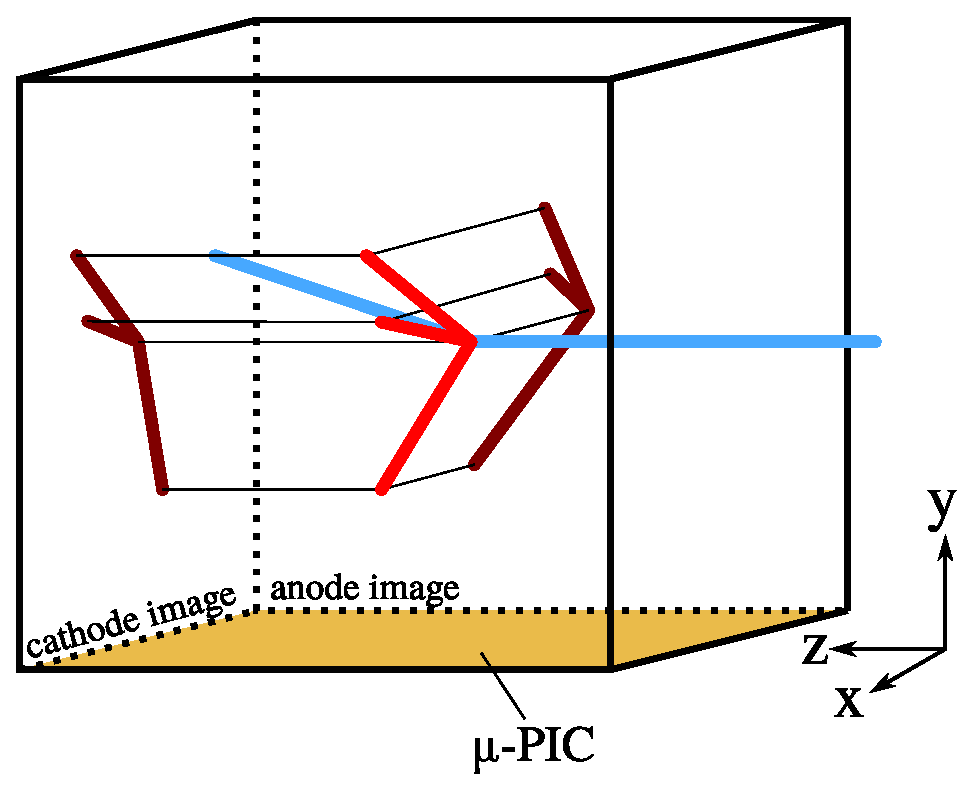
\includegraphics[clip, width=0.8\columnwidth]{MAIKo.eps}
  \caption[MAIKo TPC の概観図.]{MAIKo TPC の概観図.
    図ではTPC の中の${}^{12}\mathrm{C}$が右から入射した中性子 (青) と散乱し,
    3つの$\alpha$粒子 (赤) に崩壊した事象を表す.
    anode image ($zy$平面) と cathode image ($xy$平面) の2平面に荷電粒子のトラックが射影される.
    中性子は電荷を持たないためanode,cathode image にトラックとして検出されない.
  }
  \label{fig::MAIKo_view}
\end{figure}
\begin{figure}
  \centering
  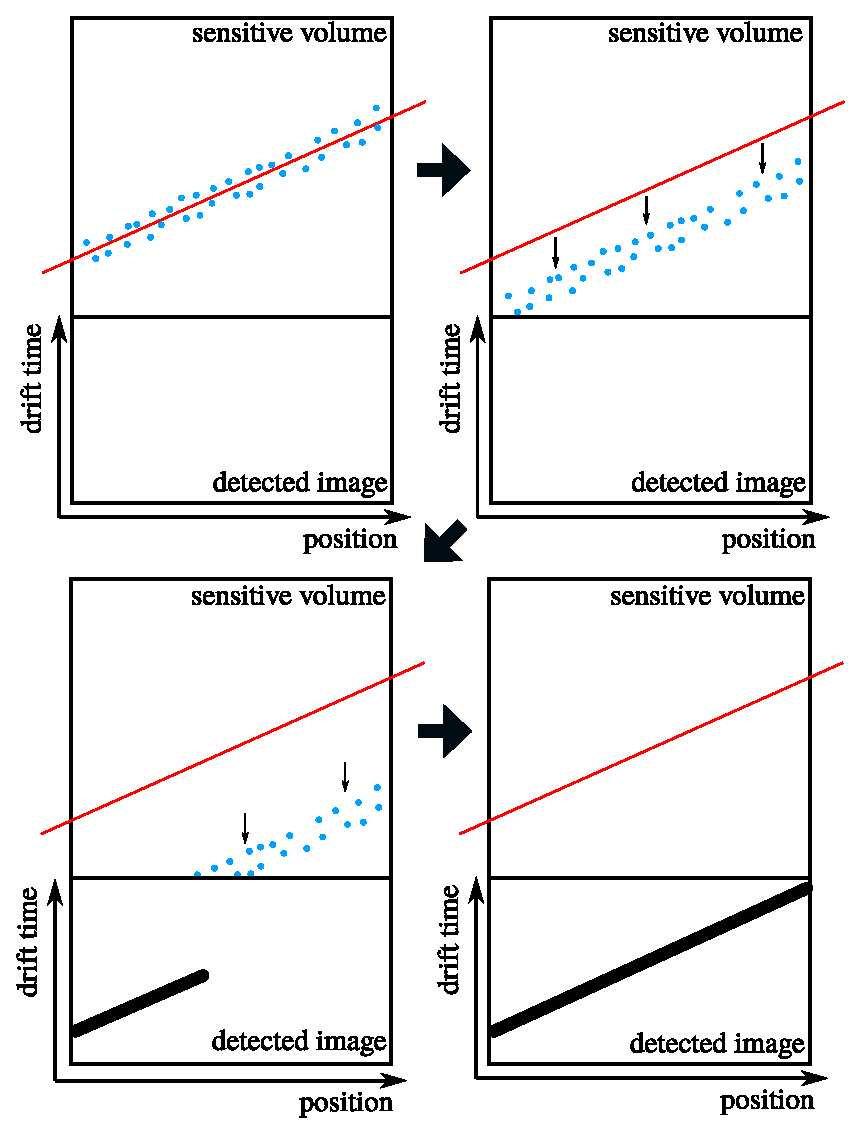
\includegraphics[clip, width=0.8\columnwidth]{drift_electrons.eps}
  \caption{TPC でトラックを検出するときのイメージ.
    赤い実線は荷電粒子のトラック,青い点はイオン化で生成された電子,
  黒く太い実線は検出されたトラックを表す.}
  \label{fig::drift_electrons}
\end{figure}
%\begin{figure}
%  \centering
%  \begin{subfigure}{0.45\columnwidth}
%    \centering
%    \includegraphics[clip, width=\columnwidth]{IMG_2925_clpd.jpg}
%    \caption{外側.}
%    \label{pic::MAIKo_chamber_out}
%  \end{subfigure}
%  \begin{subfigure}{0.45\columnwidth}
%    \centering
%    \includegraphics[clip, width=\columnwidth]{IMG_20190801_160046_clpd.jpg}
%    \caption{内側.}
%    \label{pic::MAIKo_chamber_in}
%  \end{subfigure}
%  \caption{MAIKo チェンバー.}
%  \label{pic::MAIKo_chamber}
%\end{figure}

図\ref{fig::MAIKo_cage}にドリフトケージの構造を示す.
ドリフトケージはplate,wire,grid,GEM (gas electron multiplier),$\mu$-PICからなる.
plate,grid,GEM,$\mu$-PICに高圧電源 (HV) が接続されている.
plate,wire,girdの間は\SI{10}{\mega\ohm}の抵抗で繋がれている.
GEM とHV は\SI{1}{\mega\ohm}と\SI{20}{\mega\ohm}の抵抗で繋がれている.
plateからgridの間の領域をドリフト領域,
gridから$\mu$-PICの間の領域を増幅領域,
$\mu$-PICの周囲を読み出し領域と呼ぶ.
ドリフト領域は$y$軸方向に\SI{140}{\milli\metre}であり,
読み出し面の大きさが\SI{102.4x102.4}{\milli\metre}であるので,
有感領域の大きさは\SI{102.4x102.4x140}{\milli\metre}となる.
\begin{figure}
  \centering
  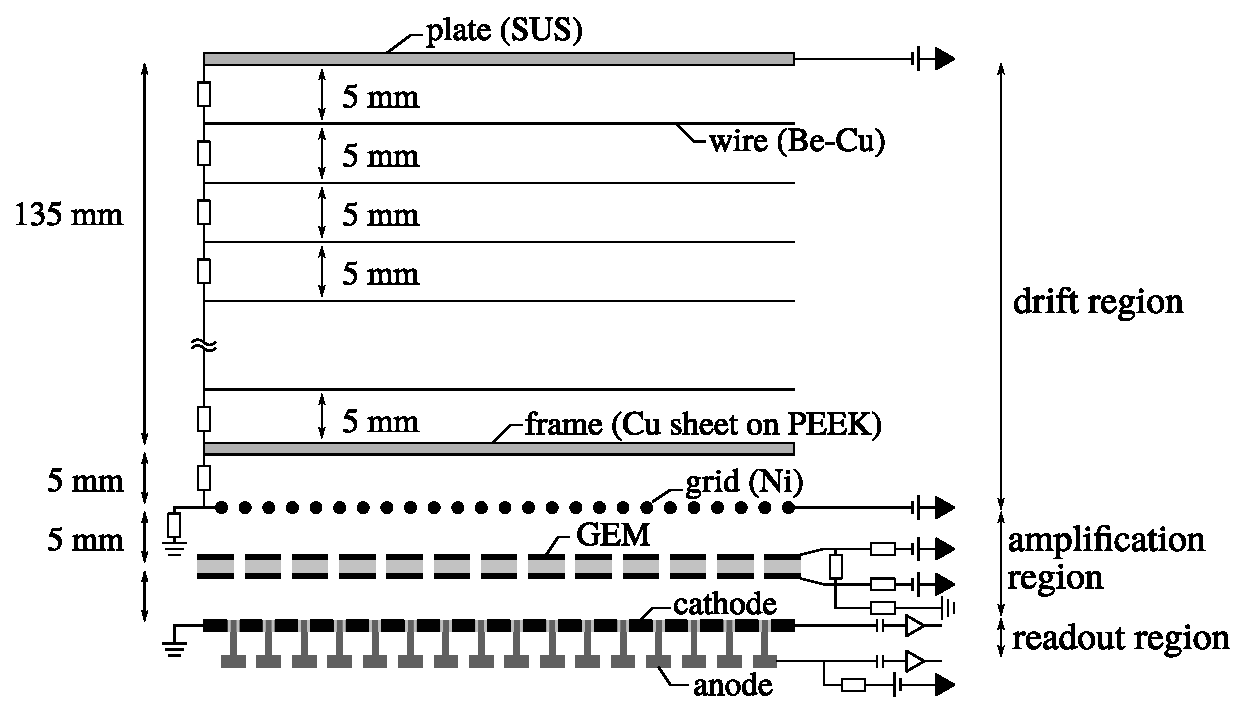
\includegraphics[clip, width=\columnwidth]{MAIKo_cage.eps}
  \caption{ドリフトケージの構造.}
  \label{fig::MAIKo_cage}
\end{figure}

%plate とgrid に電圧をかけることでドリフト領域にドリフト電場を形成する.
%ドリフト領域を荷電粒子が通過する際に生成された電子がドリフト電場によって増幅領域へ移動する.
%ドリフト電場を一様に形成するために5 mm間隔でドリフト領域の周囲にwire を巻いてある.
%ドリフト領域はドリフト方向に140 mm である.
%ドリフトしてきた電子は,まずGEM (gas electron multiplier) で増幅される.
%増幅した電子およびイオンによって$\mu$-PIC のanode とcathode に誘起された信号を読み出す.
%$\mu$-PIC では信号の読み出しだけでなく電子の増幅も行われる.

\subsection{ドリフト領域}
plate とgrid にそれぞれ高電圧を印加することでドリフト電場を形成し,
grid からplate の方向 (図\ref{fig::MAIKo_cage}では上向き) にドリフト電場を形成することで
トラックの周囲に発生した電子を増幅領域へドリフトさせる.
ドリフト電場の一様性が高いほど,トラックの周囲に発生した電子雲の形状を保ったまま,
電子をドリフトさせることができる.
均等にドリフトしない場合,正しくトラックを検出することができなくなってしまう.
ドリフト電場を一様に形成するために\SI{10}{\mega\ohm}の抵抗で接続されたwire が
\SI{5}{\milli\metre}間隔で二重で巻かれている~\cite{furuno}.

\subsection{増幅領域}
MAIKo TPC ではGEM と$\mu$-PICを用いて電子の増幅を行う.
GEM は,図\ref{pic::GEM}のようにポリマーのフィルムの表面を銅で被覆し,
直径\SI{70}{\micro\metre} の穴を\SI{140}{\micro\metre}間隔で\SI{1}{\square\milli\metre}あたり
100 個の密度で開けたものである.
銅の2つの層はポリマーによって絶縁されている.
銅の両面に電圧を印加することによって,穴の中に高電場が形成されドリフトしてきた電子が穴を通過する際に増幅される.
\begin{figure}
  \centering
  \includegraphics[clip, width=0.7\columnwidth]{gem_structure.pdf}
  \caption{GEM の拡大図~\cite{gem_compass}.}
  \label{pic::GEM}  
\end{figure}

$\mu$-PIC は京都大学宇宙線研究室で開発されたMicro Pattern Gas Detector の一種である.
$\mu$-PIC は図\ref{fig::mupic}のようにanode strip とcathode strip が直交するように配置されている.
anode strip,cathode strip ともに\SI{400}{\micro\metre}間隔でそれぞれ256~ch分割されている.
直径\SI{50}{\micro\metre}の円柱状のanode 電極に高電圧を印加し,
cathode 電極を接地することで高電場を形成することができ,
$\mu$-PICによって信号が読み出される直前に電子が増幅される.
\begin{figure}
  \centering
  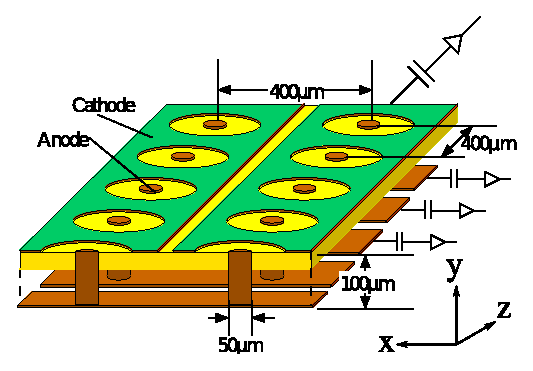
\includegraphics[clip, width=0.7\columnwidth]{upic_struc_xyz.eps}
  \caption[$\mu$-PICの概観図.]{$\mu$-PICの概観図~\cite{mupic}.
    図中の横方向にanode strip,奥行き方向にcathode strip が配置されている.
  }
  \label{fig::mupic}
\end{figure}

\subsection{読み出し領域}
\label{sec::mu-pic}
図\ref{fig::MAIKo_view}と図\ref{fig::mupic}中ではanode strip が$x$軸,cathode strip が$z$軸と平行になるように
$\mu$-PICが配置されている.
GEMと$\mu$-PICにより増幅された電子とイオンをanode strip とcathode strip により読み出すことで,
$z$座標,$x$座標を検出することができる.
また,anode strip とcathode strip で検出される信号の時間分布により$y$座標を決定することができる.

MAIKo TPC からは図\ref{fig::MAIKo_view}のようにトラックが
anode strip に垂直な面 ($zy$平面) に射影されたanode image と
cathode strip に垂直な面 ($xy$平面) に射影されたcathode image の2つの画像が取得される.
MAIKo TPC から得られる画像の1例を図\ref{fig::track_demo}に示す.
anode strip とcathode strip はそれぞれ256~chで構成され,
各ストリップの信号は\SI{100}{\mega\hertz}で1,024~samples測定し,
設定した閾値に対するtime over threshold (TOT) を取得する.
TOT は閾値以上を1,以下を0としたものである.
よって,出力されるデータは解像度が$256\times1,014$~pixels の白黒画像となる.
また,anode strip,cathode strip ともに32~chごとにまとめた信号の波形を
\SI{25}{\mega\hertz}のサンプリング率を持つFADC で取得している.
FADC で取得した信号の一例を図\ref{fig::FADC_waveform}に示す.
\begin{figure}
  \centering
  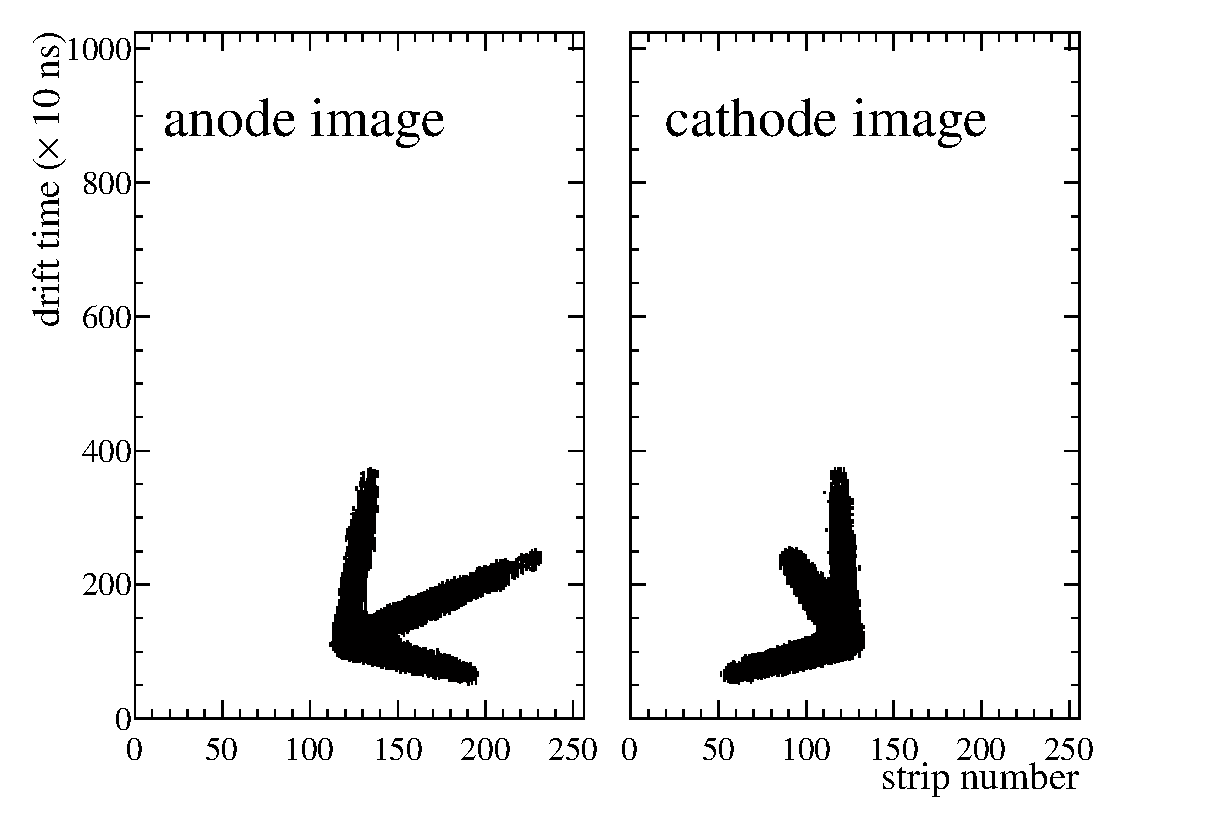
\includegraphics[clip, width=0.9\columnwidth]{10024_4.eps}
  \caption[MAIKo TPC から得られる画像データの一例.]
          {MAIKo TPC から得られる画像データの一例.
          このイベントは\ref{chap::simulation}章で述べるシミュレーションによって生成したデータである.}
  \label{fig::track_demo}
\end{figure}
\begin{figure}
  \centering
  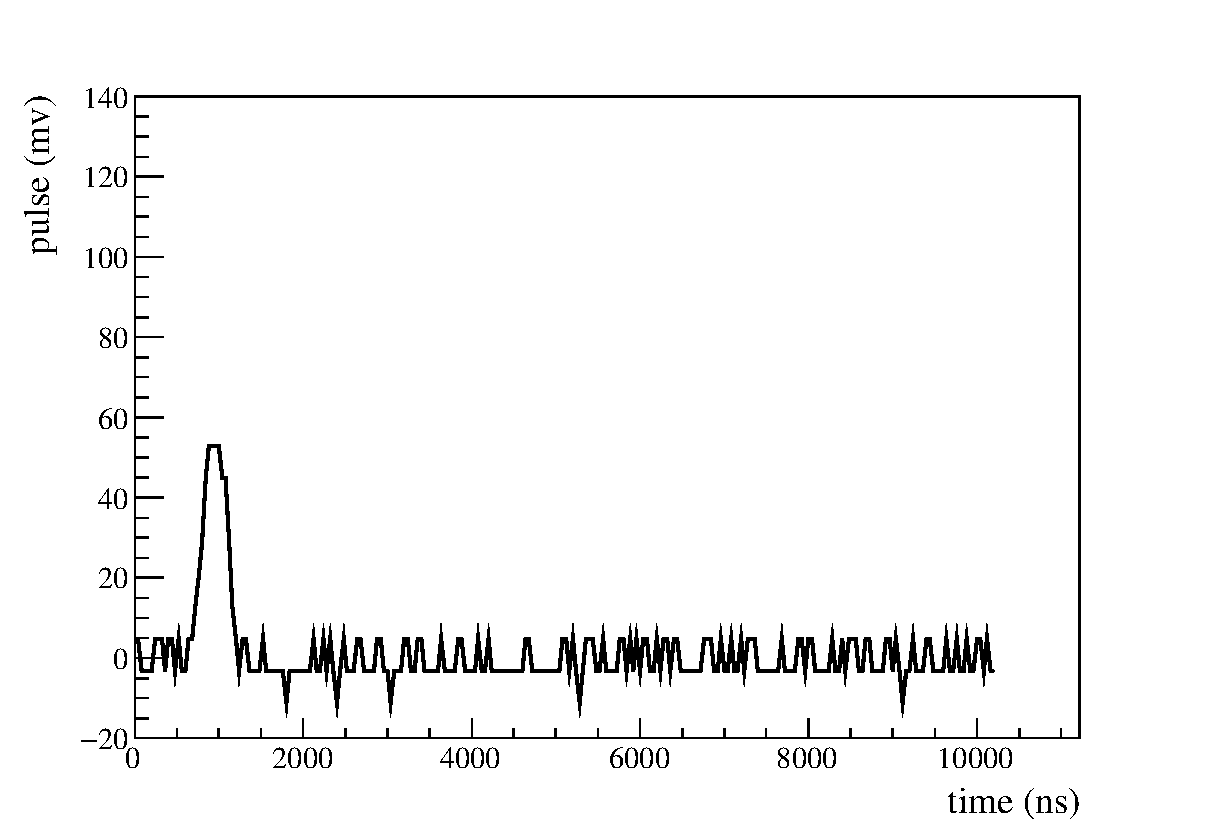
\includegraphics[clip, width=0.7\columnwidth]{0210_waveform_2.eps}
  \caption[FADCで取得された$\mu$-PICの波形の一例.]
          {FADCで取得された$\mu$-PICの波形の一例.
          この波形は\isoButaneHydro を検出ガスに用いて,$\alpha$線源でテストした際のものである.}
  \label{fig::FADC_waveform}
\end{figure}

\section{検出ガスの選出}
\label{sec::detection_gas_candidate}
標的に${}^{12}\mathrm{C}$を用いるため,分子中に炭素を含むガスを検出ガスに用いる必要がある.
${}^{12}\mathrm{C}$以外の原子核が含まれると背景事象となるが,
陽子または${}^{4}\mathrm{He}$と\SI{14}{\mega\electronvolt}の中性子の散乱では複数の荷電粒子に崩壊しないため,
トラックの本数から背景事象を取り除くことができる.
そこで,水素と炭素以外の原子が含まれない炭化水素を検出ガスに用いる.
代表的な炭化水素に,メタン (\Methane) やエタン ($\mathrm{C_{2}H_{6}}$),
イソブタン (\isoButane) がある.
また,水素ガスやヘリウムガスと炭化水素の混合ガスも用いることができる.
検出ガスとして求められる性能には以下のようなものがある.
\begin{itemize}
\item
  放電しにくい.(安定なTPC の運用)
\item
  $\alpha$粒子のエネルギー損失 ($dE/dx$) が適切である.(トラックを正しく抽出)
\item
  適切なドリフト速度を達成できる.(有感領域を効率的に使用)
\item
  電子の拡散効果が小さい.(複数のトラックを正しく抽出)
\item
  測定を行うのに十分な量の${}^{12}\mathrm{C}$を含む.(散乱標的の量)
\end{itemize}
これらの項目を基準に検出ガスの種類と圧力を決定する.

\subsection{$\alpha$粒子のエネルギー損失}
MAIKo TPC では荷電粒子のトラックの長さと方向からエネルギーと運動量を決定するため,
取得した画像からトラックを正しく抽出することが必要となる.
荷電粒子のエネルギー損失 ($dE/dx$) が大きくなりすぎると検出ガス中での飛行距離が短くなり,
トラックとして識別することが難しくなる.
また,$dE/dx$ が小さくなりすぎると荷電粒子が有感領域で停止せず,
トラックの長さを決定することができなくなる.
そこで,検出する対象である$\alpha$粒子の $dE/dx$ が適切な大きさとなるガスの種類と圧力の候補を決定する必要がある.

まず,代表的な炭化水素である\Methane を考える.
ガス中で\SI{10}{\milli\metre} 以上飛行し,MAIKo TPC の有感領域中で停止する$\alpha$粒子を検出可能な$\alpha$粒子とする.
3つの$\alpha$粒子を検出できたイベントの割合を検出率とする.
%図\ref{fig::alpha_E_dist}に示したエネルギー分布の$\alpha$粒子に対する,
図\ref{fig::sig_angle_dist}に示した微分断面積の角度分布を仮定したときの
検出率の圧力依存性を図\ref{fig::efficiency_P_dist}に示す.
ここでは,ビーム軸が有感領域の中央を通り,散乱点がビーム軸上に一様に分布していると仮定した.
図\ref{fig::efficiency_P_dist}から分かるように,\SI{50}{\hecto\pascal} で検出率が最大となっている.
%\SI{50}{\hecto\pascal}のときの\Methane の各種の値は表\ref{tab::CH4_50_params}のとおりである.
\SI{50}{\hecto\pascal}のときの\Methane の$dE/dx$と同程度となる,他の検出ガスを考え,
表\ref{tab::mixture}に示した6つを検出ガスの候補とした.
%混合ガスでは圧力を\SI{100}{\hecto\pascal} に固定し混合比をパラメータとして$dE/dx$を合わせる.
括弧内はガスの混合の割合を示す.
これらの6種類の候補から検出ガスを選ぶ.
\begin{figure}
  \centering
  \includegraphics[clip, width=0.8\columnwidth]{efficiency_P_dist.eps}
  \caption[\Methane の圧力による検出効率の分布.]
          {\Methane の圧力による検出効率の分布.
            $\alpha$粒子は図\ref{fig::sig_angle_dist}に示した微分断面積の角度分布を仮定した.
           }
  \label{fig::efficiency_P_dist}
\end{figure}
%\begin{table}
%  \centering
%  \caption{\SI{50}{\hecto\pascal}のときの\Methane のパラメータ.}
%  \label{tab::CH4_50_params}
%  \begin{tabular}{cc}
%    \toprule
%    項目 & 値\\
%    \midrule
%    密度 & \SI{3.29e-5}{\gram\per\cubic\centi\metre} \\
%    $dE/dx$ ($E_{\alpha} = \SI{0.5}{\mega\electronvolt}$, \SI{10}{\milli\metre}) & \SI{0.107}{\mega\electronvolt}\\
%    飛程 ($E_{\alpha} = \SI{0.5}{\mega\electronvolt}$) & \SI{65.6}{\milli\metre} \\
%    検出率 & \SI{48.2}{\percent} \\
%    \bottomrule
%  \end{tabular}
%\end{table}
\begin{table}
  \centering
  \caption[ガスの混合パターン,圧力,$dE/dx$.]
          {ガスの混合パターン,圧力,$dE/dx$.
            括弧内はガスの混合の割合を示す.
            エネルギー損失は$E_{\alpha}$が\SI{0.5}{\mega\electronvolt}の$\alpha$粒子が\SI{10}{\milli\metre}で
            落とすエネルギーを表す.
            電場はMagboltz による計算でドリフト速度が\SI{0.014}{\milli\metre\per\nano\second}となる値である.}
  \label{tab::mixture}
  \begin{tabular}{ccccc}
    \toprule
    gas &
    \begin{tabular}{c}
      pressure \\
      (\si{\hecto\pascal})
    \end{tabular} &
    \begin{tabular}{c}
      density \\
      (\si{\gram\per\cubic\centi\metre})
    \end{tabular} &
    \begin{tabular}{c}
      $dE/dx$ \\
      (\si{\mega\electronvolt})% \\      
%      $E_{\alpha} = \SI{0.5}{\mega\electronvolt}$% \\
%      \SI{10}{\milli\metre}
    \end{tabular} &
    \begin{tabular}{c}
      %      ドリフト電場 (\si{\volt\per\milli\metre}) \\
      電場 \\
      (\si{\volt\per\milli\metre})% \\
%      @ \SI{0.014}{\milli\metre\per\nano\second}
    \end{tabular}\\
    \midrule
    \Methane         & 50  & 3.29$\times 10^{-5}$ & 0.107 & 0.418 \\
    \MethaneHydro    & 100 & 2.55$\times 10^{-5}$ & 0.107 & 4.31 \\
    \MethaneHerium   & 100 & 3.62$\times 10^{-5}$ & 0.109 & 1.89 \\
    \isoButane       & 15  & 3.58$\times 10^{-5}$ & 0.102 & 0.644 \\
    \isoButaneHydro  & 100 & 3.13$\times 10^{-5}$ & 0.122 & 6.80 \\
    \isoButaneHerium & 100 & 3.86$\times 10^{-5}$ & 0.102 & 3.26 \\
    \bottomrule
  \end{tabular}
\end{table}

\subsection{ドリフト速度}
MAIKo TPC では\SI{100}{\mega\hertz}で1,024 samples データを取得するため,
ドリフト方向には\SI{10.24}{\micro\second}のタイムウィンドウが開いている.
ドリフトケージの大きさ (\SI{140}{\milli\metre}) を可能な限りタイムウィンドウに収めるためには,
ドリフト速度を$\SI{140}{\milli\metre}/\SI{10.24}{\micro\second} \sim \SI{0.014}{\milli\metre\per\nano\second}$
に調整する必要がある.
Magboltz~\cite{magboltz} によって求めたドリフト電場とドリフト速度の関係を図\ref{fig::drift_v_magboltz}に示す.
ドリフト速度が\SI{0.014}{\milli\metre\per\nano\second}となるドリフト電場の値を表\ref{tab::mixture}に示す.
図\ref{fig::drift_v_magboltz}の横方向の点線は\SI{0.014}{\milli\metre\per\nano\second}を表す.
以降,これらのドリフト電場で評価を行う.
\begin{figure}
  \centering
  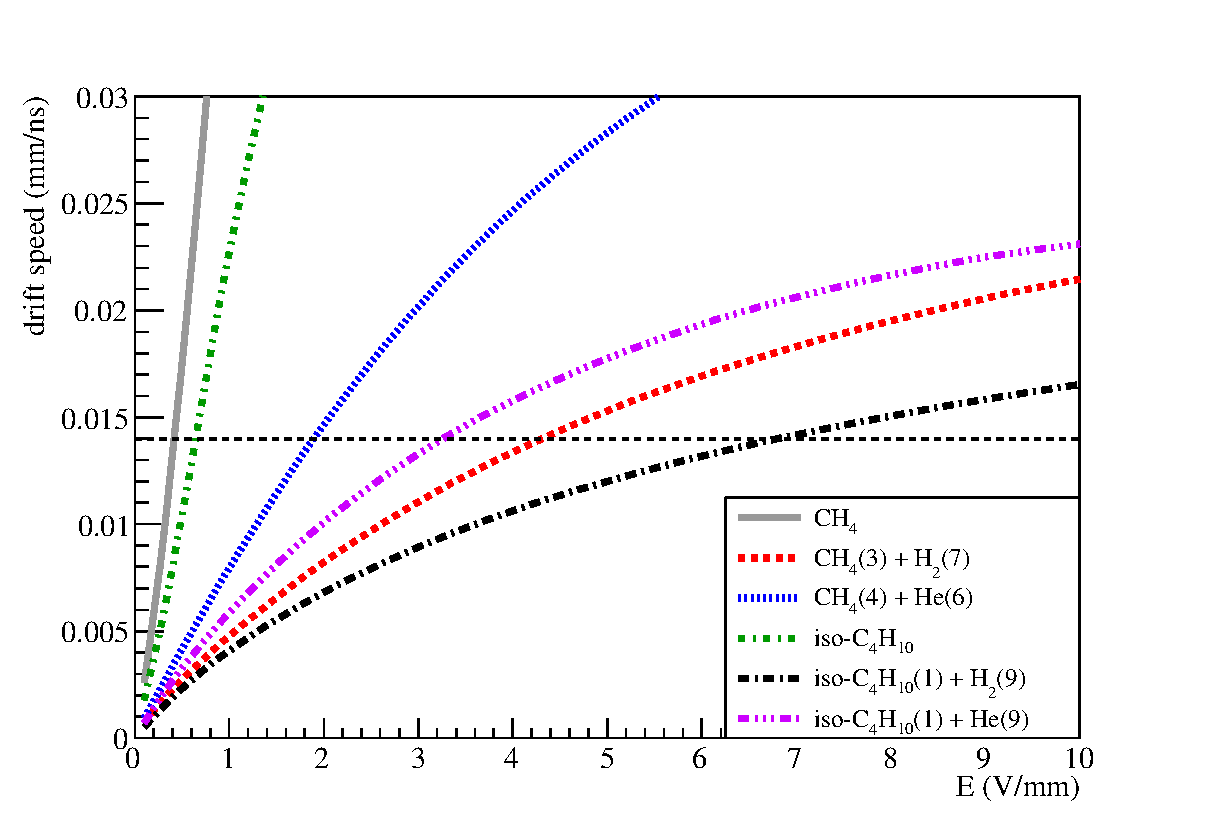
\includegraphics[clip, width=0.9\columnwidth]{drift_v_magboltz.eps}
  \caption[ドリフト電場とドリフト速度の関係.]
          {ドリフト電場とドリフト速度の関係.
            \Methane は\SI{50}{\hecto\pascal},\isoButane は\SI{15}{\hecto\pascal},その他は\SI{100}{\hecto\pascal}である.
            横方向の破線は\SI{0.014}{\milli\metre\per\nano\second}を示す.}
          \label{fig::drift_v_magboltz}
\end{figure}

\subsection{電子の拡散の効果}
ドリフト電場によって電子が移動する間に検出ガスとの散乱と電子の熱運動により,
図\ref{fig::diffusion-image}のように広がりながらドリフトする.
%電子が広がることを拡散と呼ぶ.
この効果が大きくなると,図\ref{fig::diffusion-image}の左のように
荷電粒子によって同じ場所に生成された電子が$\mu$-PICに到達するまでに広がるため,
トラックが太く検出される.
トラックが太くなると,複数のトラックを分離することが難しくなる.
そのため,図\ref{fig::diffusion-image}の右のように拡散の効果が小さいことが望まれる.
\begin{figure}
  \centering
  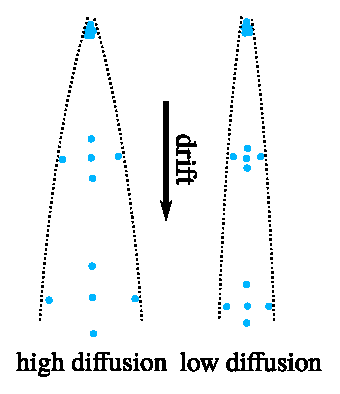
\includegraphics[clip, width=0.4\columnwidth]{diffusion_image.eps}
  \caption[電子が拡散するイメージ.]
          {電子が拡散するイメージ.
          同じ位置で生成された電子でもドリフトする間に位置が拡散する.}
  \label{fig::diffusion-image}
\end{figure}

Ref~\cite{leo}によるとドリフト電場がない場合の電子の拡散は以下のように理解できる.
電子は熱運動により発生点から拡散する.
熱運動の平均速度$v$はMaxwell 分布より
\begin{equation}
  v = \sqrt{\frac{8k_{B}T}{\pi \si{\electronmass}}}
  \label{eq::maxwell_velocity}
\end{equation}
と表せる.
ここで$k_{B}$はボルツマン定数,$T$は温度,\si{\electronmass}は電子の質量である.
電子が発生した時刻から$\Delta t$後では,
\begin{equation}
  \frac{N_0}{\sqrt{4\pi D \Delta t}}\exp\left(-\frac{x^{2}}{4 D \Delta t}\right)
  \label{eq::gaus_dist}
\end{equation}
のガウス分布で電子が広がる.
ここで$N_{0}$は全粒子数,$x$は発生した点からの距離,$D$は拡散係数を表す.
拡散係数$D$は電子の平均自由行程$\lambda$を用いて
\begin{equation}
  D = \frac{1}{3}v\lambda
  \label{eq::diffusion_coef}
\end{equation}
と表せる.
これは電子の速度が遅いほど,ガスとの散乱が少ないほど遠くまで移動できるため,
拡散の効果が大きくなることを表す.
理想気体において平均自由工程$\lambda$は,ガスとの散乱の全断面積$\sigma_{0}$,圧力$p$のもとで
\begin{equation}
  \lambda = \frac{1}{\sqrt{2}}\frac{k_{B}T}{\sigma_{0}p}
  \label{eq::lambda}
\end{equation}
と表される.
式\ref{eq::maxwell_velocity}, \ref{eq::diffusion_coef}, \ref{eq::lambda}により,
\begin{equation}
  D = \frac{2}{3\sqrt{\pi}}\frac{1}{p\sigma_{0}}\sqrt{\frac{\left(k_{B}T\right)^{3}}{\si{\electronmass}}}
  \label{eq::diffusion_coef_2}
\end{equation}
となる.
式\ref{eq::diffusion_coef_2}より,
同じガスでは圧力が高いほど,温度が低いほど拡散係数が小さいことが分かる.

ドリフト電場がある場合,発生点からの距離を$L$,ドリフト速度を$v_{\text{drift}}$とすると,
\begin{equation}
  \Delta t = \frac{L}{v_{\text{drift}}}
  \label{eq::delta_t}
\end{equation}
となる.
距離$L$における分散$\sigma(L)$は
\begin{align}
  \sigma(L) & = \sqrt{2 D \Delta t}\\
  & = \sqrt{\frac{2 D}{v_{\text{drift}}}}\times\sqrt{L}\\
  & = D_{\mathrm{Magboltz}}\times\sqrt{L}
\end{align}
となる.
計算コードMagboltz によって得られた拡散係数を表\ref{tab::diffusion}に示す.
表\ref{tab::diffusion}中の$D_{t}$はドリフト電場に対して垂直な方向への拡散,$D_{l}$は平行な方向への拡散の係数を表す.
\Methane および\isoButane の単体では拡散係数が大きく,
同じドリフト速度のとき,ドリフト電場が大きいほど拡散係数が小さいことが分かる.
\isoButaneHydro の拡散係数が最も小さく,
検出ガスの最有力候補である.
シミュレーションにより生成した${}^{12}\mathrm{C}(\mathrm{n},\mathrm{n}'){}^{12}\mathrm{C} (0_2^+)$イベントを解析し,
その解析効率により検出ガスを決定する.
\begin{table}
  \centering
  \caption[Magboltz で計算した拡散係数.]
          {Magboltz で計算した拡散係数.
            拡散の大きさはドリフト電場に依存するため,
            ここではドリフト速度が\SI{0.014}{\milli\metre\per\nano\second}になるドリフト電場での値を示す.
          $D_{t}$,$D_{l}$はそれぞれ運動方向に垂直,平行方向の拡散係数.}
  \label{tab::diffusion}
  \begin{tabular}{ccccc}
    \toprule
    gas & pressure (\si{\hecto\pascal}) & $D_{t}$ (\si{\sqrt{\milli\metre}}) & $D_{l}$ (\si{\sqrt{\milli\metre}}) &
    ドリフト電場 (\si{\volt\per\milli\metre}) \\
    \midrule
    \Methane & 50 & 0.433 & 0.547 & 0.418\\
    \MethaneHydro & 100 & 0.214 & 0.171 & 4.31\\
    \MethaneHerium & 100 & 0.270  & 0.248 & 1.89\\
    \isoButane & 15 & 0.357 & 0.414 & 0.644\\
    \isoButaneHydro & 100 & 0.196 & 0.145 & 6.80\\
    \isoButaneHerium & 100 & 0.246 & 0.197 & 3.26\\
    \bottomrule
  \end{tabular}
\end{table}

%\section{$\alpha$線源を用いた測定}
%$\alpha$線源を用いてMAIKo TPC の動作確認を行う.
%線源では,電子のドリフトスピード,増幅率,トラックの太さを確認する.

%\subsection{HV系}
%%ここでは電圧の変数名を説明する.
%
%\subsection{ガス系}
%
%\subsection{回路系}
%

%ドリフト速度の決定方法は30 degree 方向に$\alpha$線源から$\alpha$を出して,
%その飛跡がデータ上でどう見えるかで決定する.
%ドリフト速度の時間依存性も見た.

%\section{中性子カウンター (液体シンチレータ)}
%\subsection{キャリブレーション}
%\subsection{波形弁別}
%\subsection{検出効率}
%
%\section{中性子カウンター (金属箔)}
%

\end{document}

%\chapter{OKTAVIAN}
\section{OKTAVIAN}
大阪大学強力14MeV中性子工学実験装置 (OKTAVIAN) によって生成した単色中性子ビームを用いて
${}^{12}\rm{C}(n,n'){}^{12}\rm{C}(0_{2}^{+})$の断面積の測定を行う。
中性子の発生には
\begin{equation}
  t(d,{}^{4}\rm{He})n
\end{equation}
反応を用いる。
この反応を用いることにより、
およそ$14\rm{MeV}$の単色中性子を発生させることが可能となる。

コッククロフト・ワルトン型加速装置を用いることで、
デューテリウムを加速しトリチウム標的に照射する。
OKTAVIANには連続照射ラインとパルスラインの2つのビームラインがある。
パルスラインでは$1\rm{kHz}$--$2\rm{MHz}$のパルス状の
ビームを照射することができる。
ビーム電流は時間平均で$6.67\rm{p\mu A}$である。
連続照射ラインでは連続的にビームを小差hすることができ、
ビーム電流は$6.67\rm{pmA}$である。
ビームの時間情報を用いて解析を行うことが可能となるが、
パルスビームラインのトリチウム標的は実験室内にあり、
コリメートされていない中性子を用いることになる。
この場合、実験室の壁などに反跳した中性子がバックグランドになるため、
本実験には適していない。
そのため、この実験では連続照射ラインを使用する。
連続照射ラインを用いる場合、
重照射室においてデューテリウムビームをトリチウム標的に照射し、
大実験室との間にある穴から中性子ビームの取り出しを行う。

\subsection{MAIKo架台}
中性子のバックグラウンドを低減させるため、
実験装置は可能な限り取り出し穴に近づける必要がある。
しかし、取り出し穴のあるは階段上にあるため、
階段の上に実験装置を設置することとなる。

\section{中性子ビーム}
\subsection{コリメータ}
\subsection{ビーム量およびエネルギー}


\documentclass[../master]{subfiles}

%\graphicspath{{../eps/}}

\begin{document}

\chapter{シミュレーションによるトラックの再現}
\label{chap::simulation}
\section{\texorpdfstring{$\alpha$}{alpha}線源を用いた測定}
\ref{sec::detection_gas_candidate}節で考えた各検出ガスについて,
実際に$\alpha$線源から放出される$\alpha$粒子のトラックを測定した.
また,それらのデータから各ガスにおけるドリフト速度,ガスの電子増幅率,トラックの幅を決定した.
測定には${}^{241}{\rm Am}$の$\alpha$線源を用いた.
図\ref{fig::a_source_track}に$\alpha$線源のトラックの一例を示す.
図\ref{fig::a_source_track}では検出ガスに\SI{100}{\hecto\pascal}の\isoButaneHydro を用いた.
\ref{sec::detection_gas_candidate}節では6種類の候補を考えたが,
ここからは単体のiso-$\rm C_{4}H_{10}$を除いた5種類について考えていく.
これは単体の\isoButane を検出ガスに用いた場合に,
拡散係数が大きくトラックが太くなると予測されることと,
圧力が\SI{15}{\hecto\pascal}と低く安定したTPC の動作が難しいと予測されるためである.
\begin{figure}
  \centering
  \includegraphics[clip, width=0.9\columnwidth]{0210_7.eps}
  \caption[$\alpha$粒子を測定したトラックの一例.]
          {$\alpha$粒子を測定したトラックの一例.
          検出ガスには\isoButaneHydro を用いた.}
  \label{fig::a_source_track}
\end{figure}

\subsection{ドリフト速度の測定}
電子のドリフト速度を線源によって得られるトラックから実測する.
測定には図\ref{pic::alpha_collimator}のような線源コリメータを用いる.
このコリメータはアクリルで作られており,1つの\ang{0}と4つの\ang{30}の穴が設けられている.
このコリメータを用いることで$\alpha$線の放出方向を\ang{0}と\ang{30}の方向に限定することができる.
\ang{30}方向の$\alpha$線は図\ref{fig::drift_v_image}の右のようにドリフト方向に$\Delta y$~\si{\milli\metre},
それと垂直な方向に$\Delta z$~\si{\milli\metre}移動するとき,
\begin{equation}
  \Delta y = \tan(\ang{30})\times\Delta z \label{eq::deltay_deltaz}
\end{equation}
となる.
MAIKo TPC で取得したトラックの横方向の変分を$\Delta strip$,縦方向の変分を$\Delta t$~\si{\nano\second},
ドリフト速度を$v_{\text{drift}}$~\si{\milli\metre\per\nano\second}とすると,
\begin{align}
  \frac{\Delta z}{\SI{0.4}{\milli\metre}} & = \Delta strip \label{eq::deltaz}\\
  \frac{\Delta y}{v_{\text{drift}}} & = \Delta t \label{eq::deltay}
\end{align}
という関係にある.
式\eqref{eq::deltay_deltaz}, \eqref{eq::deltaz}, \eqref{eq::deltay} より
\begin{equation}
  v_{\text{drift}} = \frac{\tan(\ang{30})\times\Delta strip\times\SI{0.4}{\milli\metre}}{\Delta t}
\end{equation}
とドリフト速度が決定される.
\begin{figure}
  \centering
  \begin{subfigure}{0.45\columnwidth}
    \centering
    \includegraphics[clip, width=0.8\columnwidth]{image30580-min.png}
    \caption{側面.}
  \end{subfigure}
  \begin{subfigure}{0.45\columnwidth}
    \centering
    \includegraphics[clip, width=0.8\columnwidth]{IMG_20191225_183542_clip.jpg}
    \caption{正面.}
  \end{subfigure}
  \caption[線源コリメータ.]
          {線源コリメータ.中央に\ang{0},上下左右に\ang{30}の穴が設けられている.
            \ang{0}の穴と1つの\ang{30}の穴を除いてカプトンテープで封じることにより,
            $\alpha$先の放出方向を限定している.
          }
          \label{pic::alpha_collimator}
\end{figure}
\begin{figure}
  \centering
  \begin{minipage}{0.45\columnwidth}
    \centering
    \includegraphics[clip, width=0.9\columnwidth]{drift_v_source.eps}
  \end{minipage}
  \begin{minipage}{0.45\columnwidth}
    \centering
    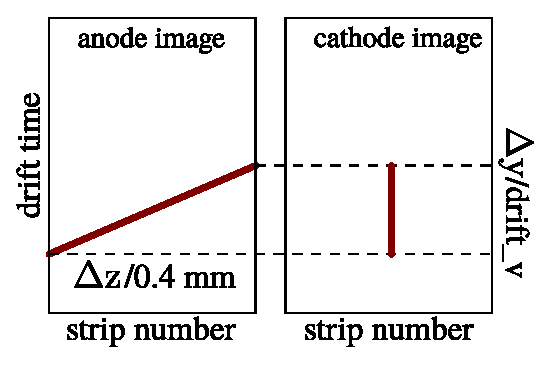
\includegraphics[clip, width=\columnwidth]{drift_v_image.eps}
  \end{minipage}
  \caption[\ang{30}に方向を限定した$\alpha$線と取得される画像データのイメージ.]
          {\ang{30}に方向を限定した$\alpha$線 (左) と取得される画像データ (右) のイメージ.}
  \label{fig::drift_v_image}
\end{figure}

$\alpha$線源を用いて測定したドリフト速度とMagboltz で計算した値を
表\ref{tab::drift_speed_compare}に示す.
コリメータの穴は有限の大きさを持つため,測定したドリフト速度の分布も有限の広がりを持つ.
ここでは,ドリフト速度の分布に対してガウス分布でフィットした結果の標準偏差を誤差とした.
$\alpha$線源を用いて測定したドリフト速度と Magboltz を用いて計算したドリフト速度が概ね一致していることが分かる.
ここで,Magboltz の計算値が\SI{0.014}{\milli\metre\per\nano\second}となっていないのは,
MAIKo TPC の実際の運用を簡単にするために設定電圧を切りの良い値にしたためである.
\Methane は実測とMagboltz による計算値に不一致が見られるが,
\Methane のみ\SI{50}{\hecto\pascal} とその他のガスと比較して圧力が半分であるため,
不純物,特に水分の影響を強く受けていると考えられる.
水分のドリフト速度へ与える影響は付録\ref{app::drift_speed_humid_dep}で述べる.
\begin{table}
  \centering
  \caption{実測したドリフト速度とMagboltz を用いて計算したドリフト速度の比較.}
  \label{tab::drift_speed_compare}
  \begin{tabular}{cccc}
    \toprule
    gas & ドリフト電場 (\si{\volt\per\milli\metre}) & 実測値 (\si{\milli\metre\per\nano\second})
    & 計算値 (\si{\milli\metre/\nano\second})\\
    \midrule
    \Methane & 0.429 & $0.0126\pm0.000825$ & 0.0145 \\
    \MethaneHydro & 4.32 & $0.0140\pm0.000809$ & 0.0140 \\
    \MethaneHerium & 1.89 & $0.0135\pm0.000832$ & 0.0140 \\
    \isoButaneHydro & 6.82 & $0.0137\pm0.000823$ & 0.0140 \\
    \isoButaneHerium & 3.29 & $0.0139\pm0.000842$ & 0.0141 \\
    \bottomrule
  \end{tabular}
\end{table}
%\begin{figure}
%  \centering
%  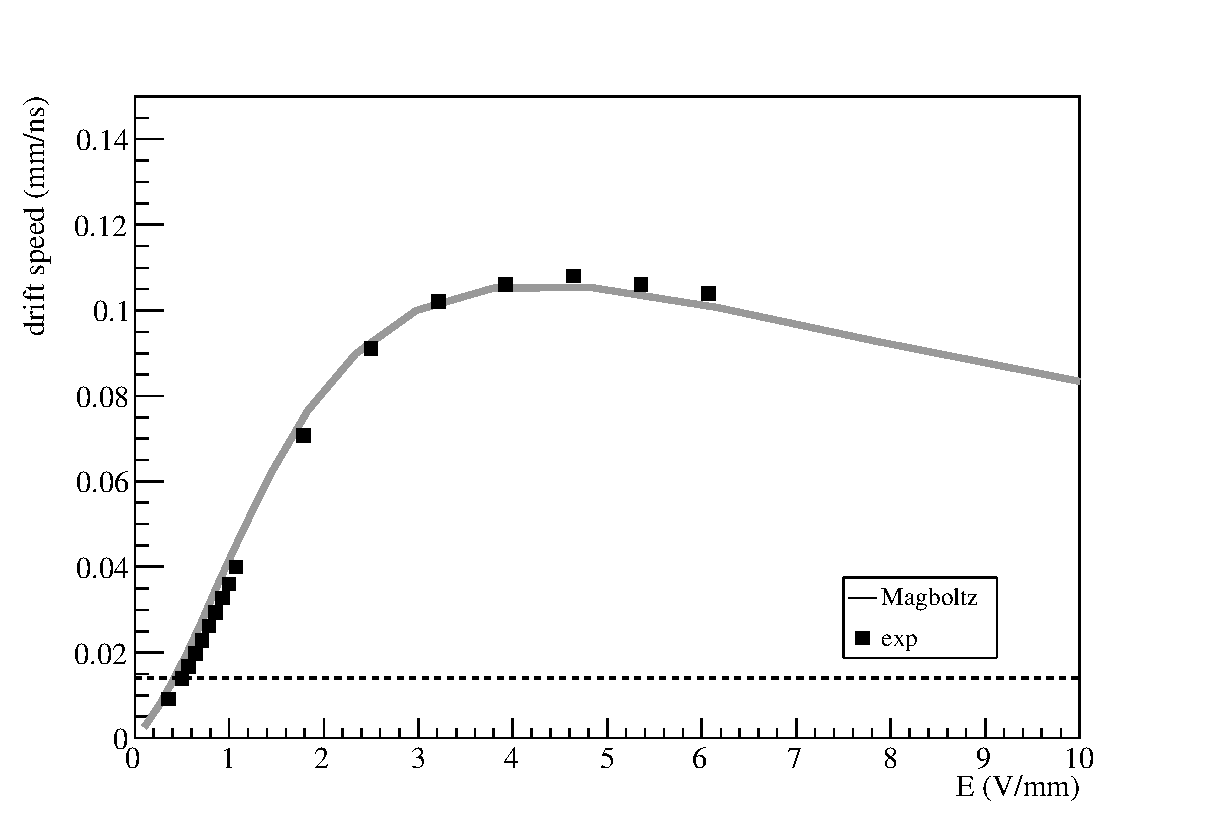
\includegraphics[clip, width=0.9\columnwidth]{drift_v_CH4.eps}
%  \caption[検出ガスに${\rm CH_{4}}$を用いたときのドリフトスピードの電場依存性.]
%          {検出ガスに${\rm CH_{4}}$を用いたときのドリフトスピードの電場依存性.
%            図中の点線は0.014 mm/ns を示す.}
%  \label{fig::drift_v_CH4}
%%  \includegraphics[clip, width=0.7\columnwidth]{drift_v_CH4_H2.eps}
%  \caption{}
%  \label{fig::drift_v_CH4_H2}
%%  \includegraphics[clip, width=0.7\columnwidth]{drift_v_CH4_He.eps}
%  \caption{}
%  \label{fig::drift_v_CH4_He}
%  \includegraphics[clip, width=0.9\columnwidth]{drift_v_iC4H10_H2.eps}
%  \caption[検出ガスにiso-${\rm C_{4}H_{10}}$を用いたときのドリフトスピードの電場依存性.]
%          {検出ガスにiso-${\rm C_{4}H_{10}}$を用いたときのドリフトスピードの電場依存性.
%        p    図中の点線は0.014 mm/ns を示す.}
%  \label{fig::drift_v_iC4H10_H2}
%%  \includegraphics[clip, width=0.7\columnwidth]{drift_v_iC4H10_He.eps}
%  \caption{}
%  \label{fig::drift_v_iC4H10_He}
%\end{figure}

\subsection{電子増幅率}
%各部の電圧に対する電子増幅率の依存性を測定した.
GEM および$\mu$-PICによる電子の増幅率を測定した.
増幅率は荷電粒子が検出ガス中を通過した際に発生させた電子数 ($N_{\mathrm{e}}$) と
増幅後に$\mu$-PICによって収集された電子数 ($N'_{\mathrm{e}}$) から求めることができる.
$N_{\mathrm{e}}$は検出ガス中での荷電粒子のエネルギー損失と検出ガスのW値(1つの電子対の生成に必要なエネルギー)から求める.
$N'_{\mathrm{e}}$は$\mu$-PICで収集した電荷から求める.
%詳しい計算方法について以下で述べる.
%
検出ガス中で荷電粒子がエネルギーを損失すると,W値あたり平均1個の電子を電離する.
そのため,荷電粒子のエネルギー損失をW値で除することで$N_{\mathrm{e}}$が求まる.
各検出ガスにおけるエネルギー損失とW値~\cite{energy_per_ion_pair,pdg}を表\ref{tab::energy_loss_and_W_val}に示す.
本研究ではでは${}^{241}\mathrm{Am}$からの$\alpha$線を用いて測定を行った.
${}^{241}\mathrm{Am}$からは\SI{5.48}{\mega\electronvolt}の$\alpha$線が放出される.
今回の測定に用いた$\alpha$線源は線量を大きくするために,多くの${}^{241}\mathrm{Am}$が線源に含まれている.
そのため,物質厚が大きくなっており,$\alpha$線が放出される前に線源中でエネルギーを損失してしまう.
この線源から出ている$\alpha$粒子の持つエネルギーが平均\SI{4.2}{\mega\electronvolt}であることが過去の測定により確認している.
今回の測定では\ang{0}方向に放出された$\alpha$線を用いて測定した.
エネルギー損失は\SI{4.2}{\mega\electronvolt}の$\alpha$粒子が$\mu$-PIC 32 strip分の
距離 (\SI{12.8}{\milli\metre}) で落とすエネルギーを示している.
この距離で発生した電子が$\mu$-PIC の32 stripsで収集される.
\begin{table}
  \centering
  \caption[検出ガスのW値とエネルギー損失と$N_{\rm e}$.]
          {検出ガスのW値~\cite{energy_per_ion_pair,pdg}とエネルギー損失と$N_{\rm e}$.
          エネルギー損失は\SI{4.2}{\mega\electronvolt}の$\alpha$粒子が
          ガス中を\SI{12.8}{\milli\metre} 進んだ時の値である.}
  \label{tab::energy_loss_and_W_val}
  \begin{tabular}{cccc}
    \toprule
    gas & W値 (\si{\electronvolt}) & energy loss (\si{\kilo\electronvolt}) & $N_{\rm e}$\\
    \midrule
    \Methane         & 29.1 & 56.5 & 1.94$\times 10^{3}$ \\
    \MethaneHydro    & 34.2 & 53.4 & 1.56$\times 10^{3}$ \\
    \MethaneHerium   & 39.2 & 59.3 & 1.51$\times 10^{3}$ \\
%    iso-${\rm C_{4}H_{10}}$                 & 26.0 & 0.0552 & 2.12$\times 10^{3}$ \\
    \isoButaneHydro  & 35.4 & 62.0 & 1.75$\times 10^{3}$ \\
    \isoButaneHerium & 44.0 & 58.0 & 1.32$\times 10^{3}$ \\
    \bottomrule
  \end{tabular}
\end{table}

32 strips まとめた$\mu$-PICからの信号波形は図\ref{fig::FADC_waveform}のようなFADC 情報として取得している.
この信号波形を時間で積分することによって32 strips で収集した電荷量を計算することができる.
$\mu$-PICで取得した電気信号は読み出し回路内部で800倍に増幅され,
FADC の入力インピーダンス\SI{50}{\ohm}で電流値を電圧値に変換して取得している.
よって,式\eqref{eq::N'e}で$\mu$-PICで収集した電荷量を得ることができる.
\si{\elementarycharge}は電気素量である.
\begin{equation}
  N'_{\mathrm{e}} = \frac{\int V (t) dt}{ 50 \times 800 \times \si{\elementarycharge}}
  \label{eq::N'e}
\end{equation}
各検出ガスの増幅率と電子の収集効率を畳み込んだ値を表\ref{tab::multiplying_rate}に示す.
ここでは,GEMと$\mu$-PIC の両方による増幅率となっている.
増幅率の分布をガウス分布でフィットした結果の標準偏差を誤差とした.
また,測定時のGEM や$\mu$-PICに印加した電圧を表\ref{tab::high_voltage_config_for_gain_meas}に示す.
\begin{table}
  \centering
  \caption{各検出ガスの電子増幅率.}
  \label{tab::multiplying_rate}
  \begin{tabular}{cc}
    \toprule
    gas & 増幅率 (倍) \\
    \midrule
    \Methane         & $700\pm114$ \\
    \MethaneHydro    & $354\pm54$ \\
    \MethaneHerium   & $322\pm69$ \\
    \isoButaneHydro  & $272\pm55$ \\
    \isoButaneHerium & $392\pm47$ \\
    \bottomrule
  \end{tabular}
\end{table}
\begin{table}
  \caption{電子増幅率を測定した際の電圧設定.GEM のうちgrid 側をGEMt,$\mu$-PIC側をGEMbとする.}
  \label{tab::high_voltage_config_for_gain_meas}
  \centering
  \begin{tabular}{cccccc}
    \toprule
    gas & plate (\si{\volt}) & grid (\si{\volt}) & GEMt (\si{\volt}) & GEMb (\si{\volt}) & $\mu$-PIC (\si{\volt}) \\
    \midrule
    \Methane         & $-1370$ & $-1290$ & $-560$ & $-150$ & $175$ \\
    \MethaneHydro    & $-2105$ & $-1500$ & $-620$ & $-250$ & $420$ \\
    \MethaneHerium   & $-1465$ & $-1200$ & $-600$ & $-250$ & $400$ \\
    \isoButaneHydro  & $-2255$ & $-1300$ & $-600$ & $-250$ & $400$ \\
    \isoButaneHerium & $-1430$ & $-970$ & $-600$ & $-250$ & $300$ \\
    \bottomrule
  \end{tabular}
\end{table}

\subsection{トラックの幅}
本実験の目的である3$\alpha$に崩壊するイベントでは観測されるトラックが太いと複数のトラックの区別が難しくなり,
トラックを正しく抽出できなくなる.
そこで,\ang{0}の$\alpha$粒子によるトラックの幅を測定した.
図\ref{fig::track_width}に示すように,
ドリフト方向のトラックの幅には\ang{0}方向に放出された$\alpha$粒子のトラックのanode image の128~strip目のclock方向の幅を,
垂直方向の幅には\ang{30}方向に放出された$\alpha$粒子のトラックのcathode image の200~clock目のstrip方向の幅を用いる.
このようにして決定したトラックの幅とMagboltz を用いて計算した拡散係数を%表\ref{tab::track_width},
図\ref{fig::diffusion_compare}に示す.
図\ref{fig::diffusion_compare}から分かるようにトラックの幅と拡散係数には正の相関がある.
拡散係数,トラックの幅ともに\isoButaneHydro が最も小さいことが分かる.
\begin{figure}
  \centering
  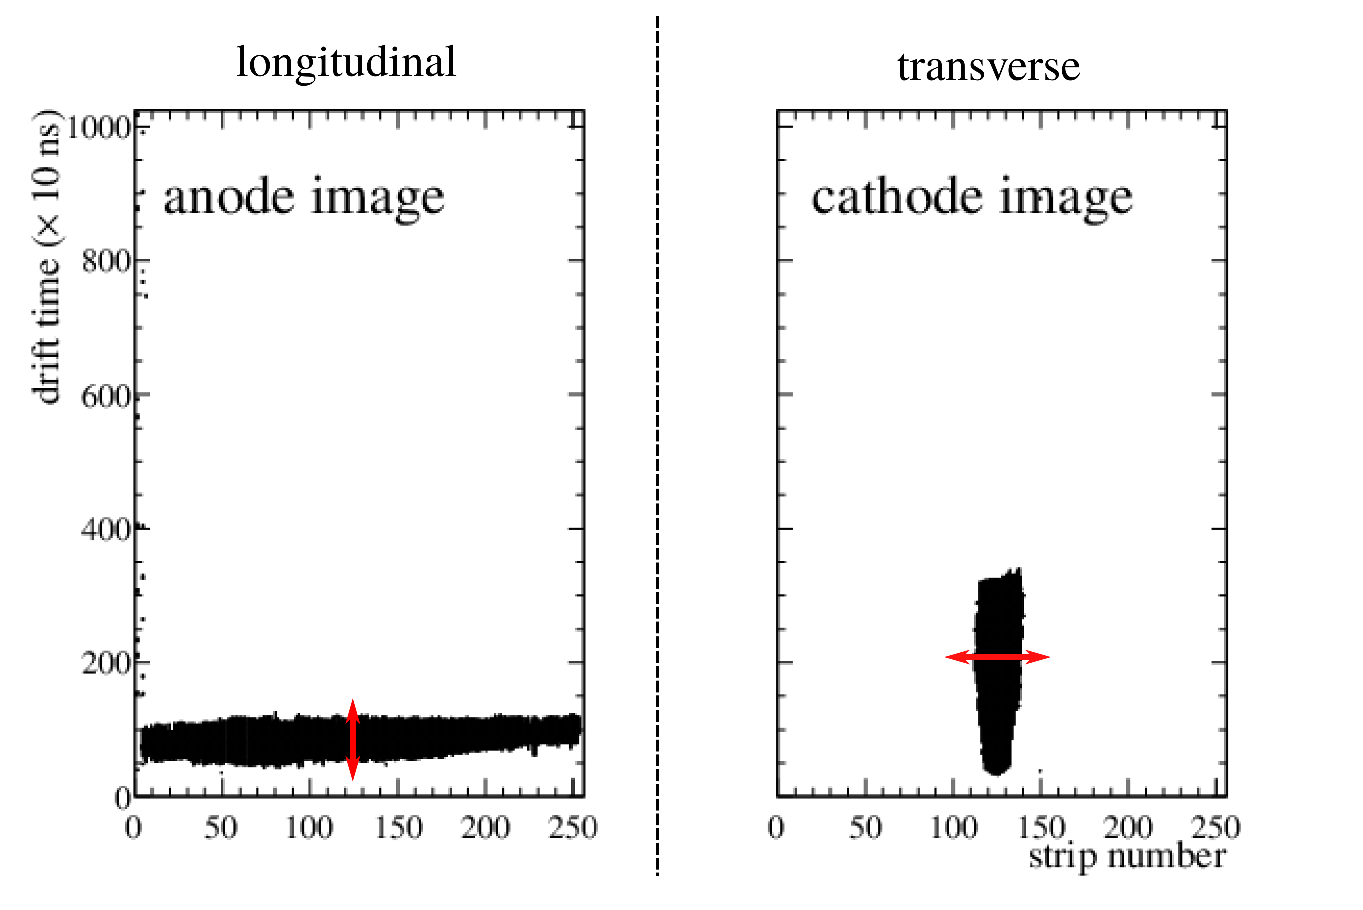
\includegraphics[clip, width=0.5\columnwidth]{track_width_2.eps}
  \caption{トラックの幅の決定方法のイメージ.
    ドリフト方向の幅にはanode image の128~strip目(左),垂直方向のトラックの幅はcathode image の200~clock目の幅を用いる.}
  \label{fig::track_width}
\end{figure}

%\begin{table}
%  \centering
%  \caption{各検出ガスでのトラックの幅.}
%  \label{tab::track_width}
%  \begin{tabular}{cc}
%    \toprule
%    gas & トラックの幅 ($\times \SI{10}{\nano\second}$)\\
%    \midrule
%    \Methane         & 91.1 \\
%    \MethaneHydro    & 42.3 \\
%    \MethaneHerium   & 62.5 \\
%    \isoButaneHydro  & 35.4 \\
%    \isoButaneHerium & 54.9 \\
%    \bottomrule
%  \end{tabular}
%\end{table}
\begin{figure}
  \centering
  \begin{subfigure}{0.45\columnwidth}
    \centering
    \includegraphics[clip, width=\columnwidth]{diffusion_track_l.eps}
    \caption{ドリフト方向に対して平行な方向.}
    \label{fig::diffusion_compare_l}
  \end{subfigure}
  \begin{subfigure}{0.45\columnwidth}
    \centering
    \includegraphics[clip, width=\columnwidth]{diffusion_track_t.eps}
    \caption{ドリフト方向に対して垂直な方向.}
    \label{fig::diffusion_compare_t}
  \end{subfigure}
  \caption{Magboltz で計算した拡散係数と実測によるトラックの幅.}
  \label{fig::diffusion_compare}
\end{figure}

\section{シミュレーションによる線源データの再現}
MAIKo TPC から得られるトラックをGarfield++~\cite{garfield++}と
Magboltz~\cite{magboltz},SRIM~\cite{SRIM}を用いたシミュレーションによりMAIKo TPC で測定されるトラックの再現を試みた.
シミュレーションでは,ドリフト電場,W値,電子増幅率,検出ガスの密度を固定した上で,
最もよく測定結果を再現する信号の閾値を探索した.
電子増幅率は$\alpha$線源を用いた測定値を用いた.
シミュレーションは以下の手順%(図\ref{fig::simulation_flow})
で行った.
\begin{enumerate}
\item\label{sim::particle_generate}
  トラックを生成する荷電粒子のエネルギー,運動量を決定し,
  Garfield++のSrimTrack に登録する.
\item
  SrimTrack によりトラックの周囲に電子を生成する.
\item
  電子をMagboltz で求めたドリフト速度と拡散係数に基づき読み出し領域へドリフトさせる.
\item
  電子のドリフト時間を信号処理回路の応答関数で畳み込む.
  すなわち,読み出し領域に到達した電子1つにつき図\ref{fig::mu-pic_readout}に示すような電気信号を
  各strip の信号波形に加算する.
\item
  設定した信号波形の閾値に基づき,信号波形を白黒画像に変換しanode image とcathode image を生成する.
\end{enumerate}
$\alpha$線源を用いた場合のシミュレーションと測定の比較を以下に示す.
図\ref{fig::track_comp_ch4}は\SI{50}{\hecto\pascal}の\Methane におけるトラック,
図\ref{fig::track_comp_ch4_h2}は\SI{100}{\hecto\pascal}の\MethaneHydro におけるトラック,
図\ref{fig::track_comp_ch4_he}は\SI{100}{\hecto\pascal}の\MethaneHerium におけるトラック, 
図\ref{fig::track_comp_ic4h10_h2}は\SI{100}{\hecto\pascal}の\isoButaneHydro におけるトラック,
図\ref{fig::track_comp_ic4h10_he}は\SI{100}{\hecto\pascal}の\isoButaneHerium におけるトラックである.
これらの$\alpha$線は図\ref{fig::drift_v_image}のように有感領域を貫通している.
信号の閾値を\SI{0.1}{\milli\volt}とすると,それぞれの検出ガスでの$\alpha$線源によるトラックを,
シミュレーションで再現できる.
\begin{figure}
  \centering
  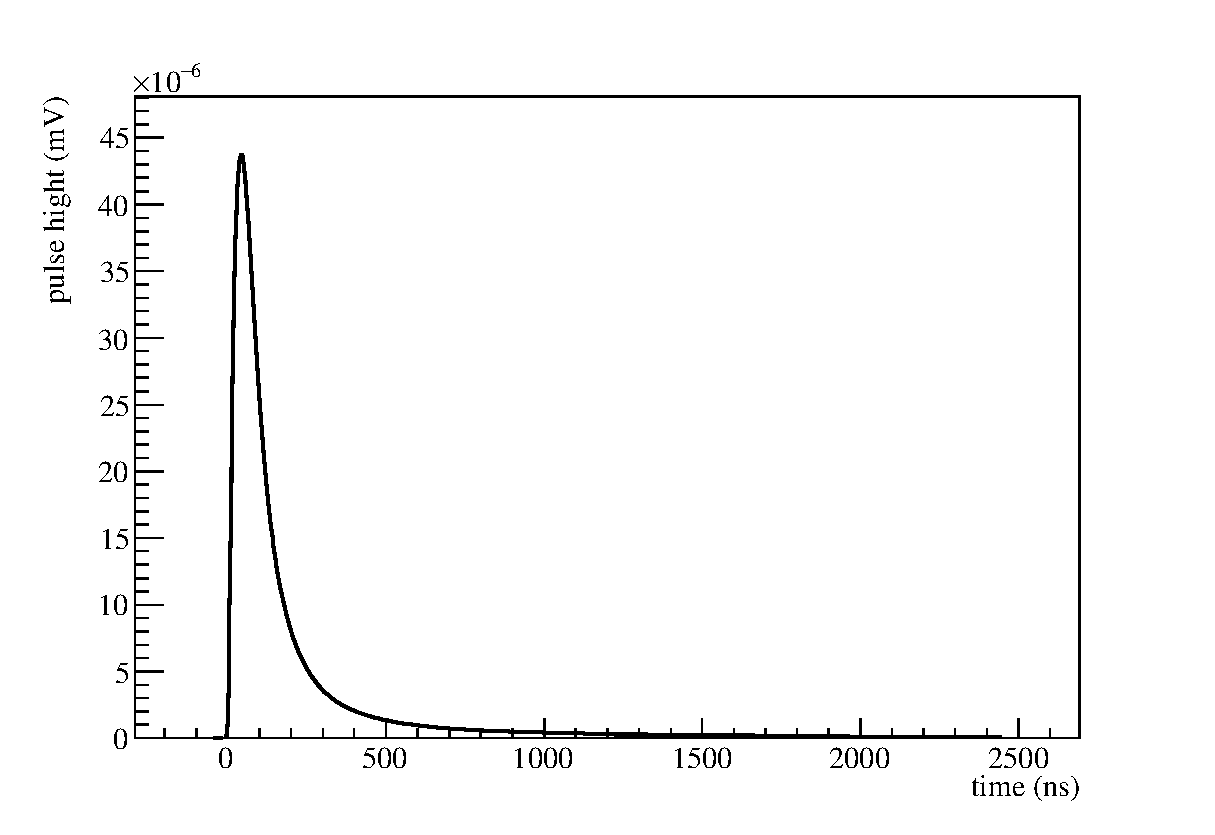
\includegraphics[clip, width=0.9\columnwidth]{waveform.eps}
  \caption{1電子が$\mu$-PICに到達した時に読み出される電気信号.}
  \label{fig::mu-pic_readout}
\end{figure}

\begin{figure}
  \centering
  \begin{subfigure}{0.48\columnwidth}
    \centering
    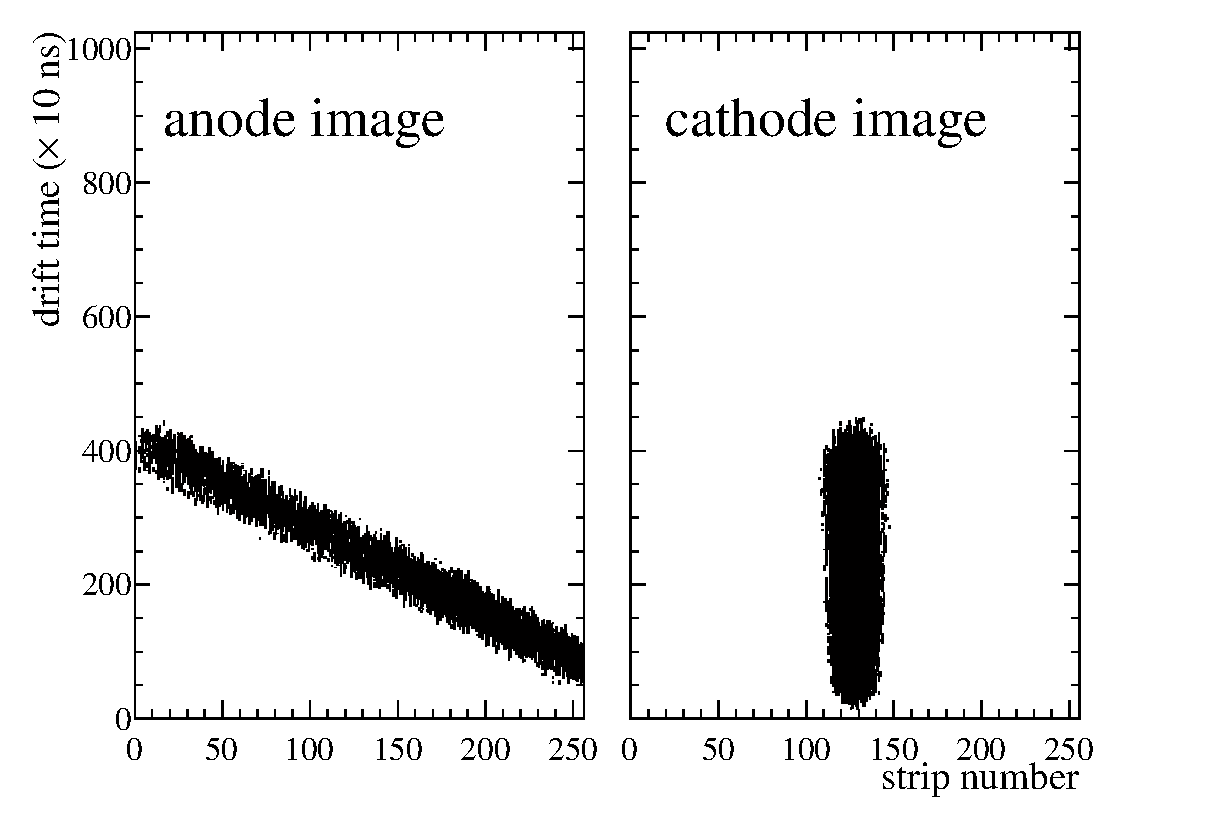
\includegraphics[clip, width=\columnwidth, trim=0 0 50 0]{CH4_0.eps}
    \caption{シミュレーションによるトラック.}
  \end{subfigure}
  \begin{subfigure}{0.48\columnwidth}
    \centering
    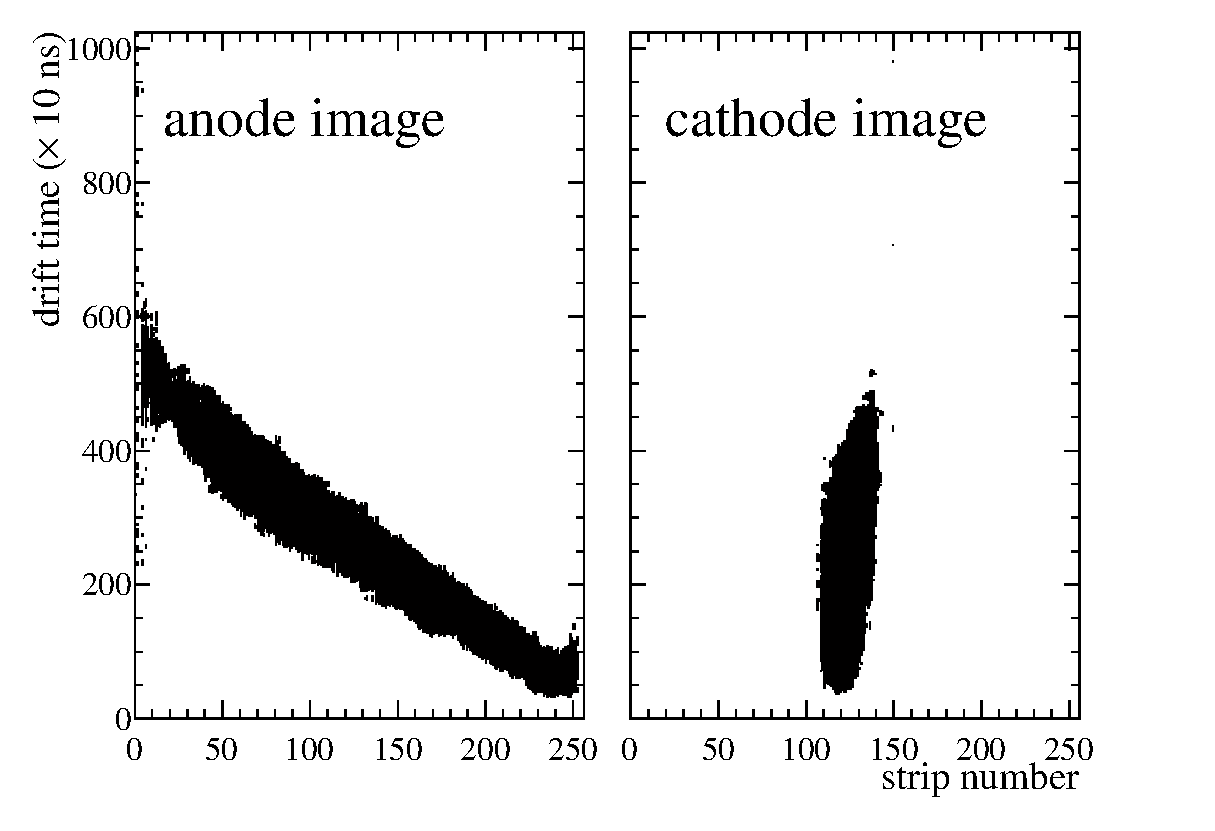
\includegraphics[width=\columnwidth, trim=0 0 50 0]{0160_5.eps}
    \caption{$\alpha$線源によるトラック.}
  \end{subfigure}
  \caption{$\alpha$粒子のトラック(\Methane の場合).}
  \label{fig::track_comp_ch4}
\end{figure}

\begin{figure}
  \centering
  \begin{subfigure}{0.48\columnwidth}
    \centering
    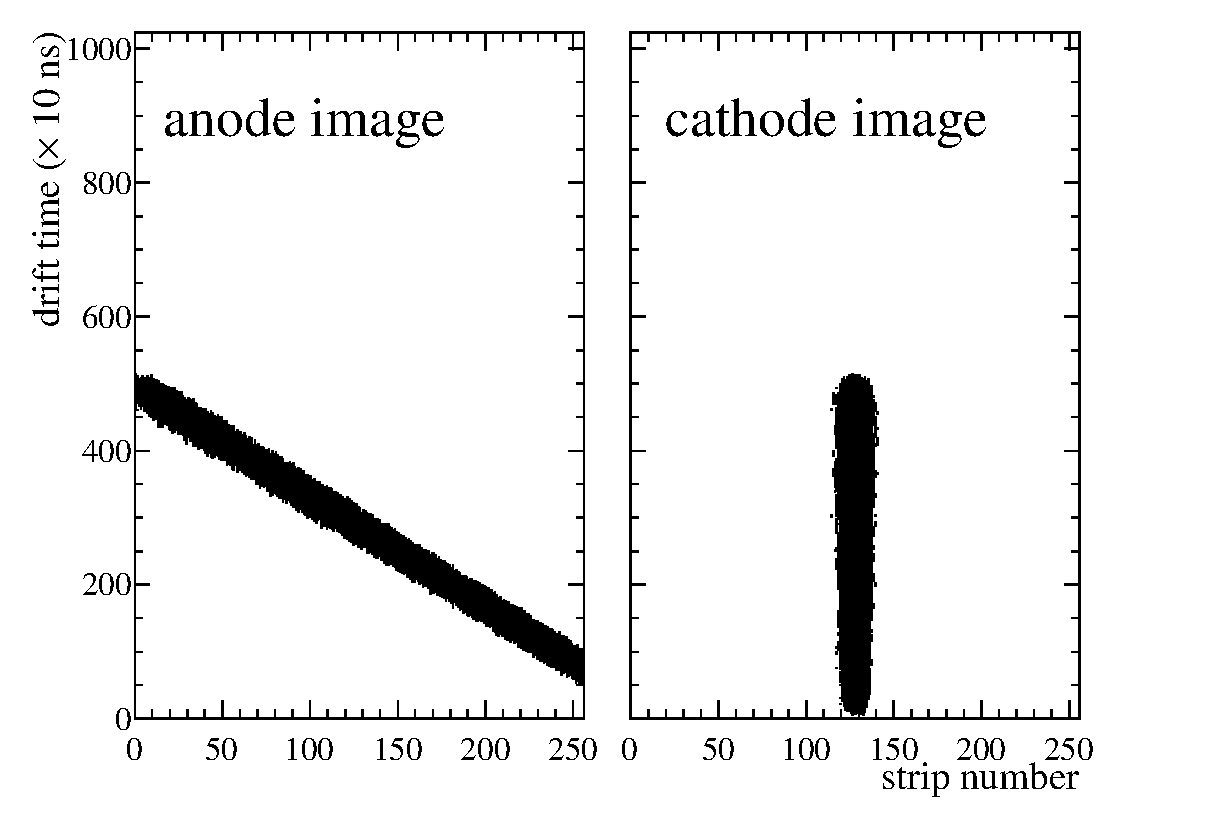
\includegraphics[clip, width=\columnwidth, trim=0 0 50 0]{CH4_3_H2_7_0.eps}
    \caption{シミュレーションによるトラック.}
  \end{subfigure}
  \begin{subfigure}{0.48\columnwidth}
    \centering
    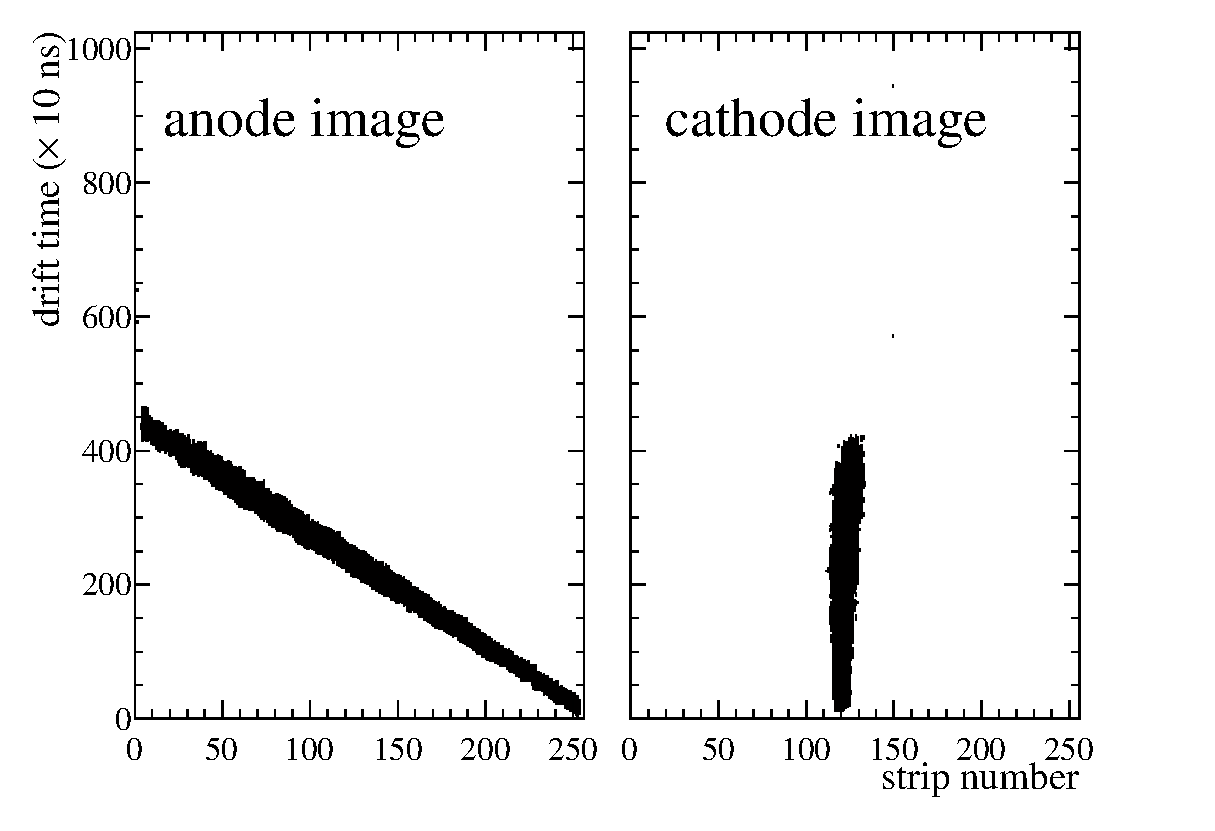
\includegraphics[clip, width=\columnwidth, trim=0 0 50 0]{0207_7.eps}
    \caption{$\alpha$線源によるトラック.}
  \end{subfigure}
  \caption{$\alpha$粒子のトラック(\MethaneHydro の場合).}
  \label{fig::track_comp_ch4_h2}
\end{figure}

\begin{figure}
  \centering
  \begin{subfigure}{0.48\columnwidth}
    \centering
    \includegraphics[clip, width=\columnwidth, trim=0 0 50 0]{CH4_4_He_6_0.eps}
    \caption{シミュレーションによるトラック.}
  \end{subfigure}
  \begin{subfigure}{0.48\columnwidth}
    \centering
    \includegraphics[clip, width=\columnwidth, trim=0 0 50 0]{0163_3.eps}
    \caption{$\alpha$線源によるトラック.}
  \end{subfigure}
  \caption{$\alpha$粒子のトラック [\MethaneHerium の場合].}
  \label{fig::track_comp_ch4_he}
\end{figure}

\begin{figure}
  \centering
  \begin{subfigure}{0.48\columnwidth}
    \centering
    \includegraphics[clip, width=\columnwidth, trim=0 0 50 0]{iC4H10_1_H2_9_0.eps}
    \caption{シミュレーションによるトラック.}
  \end{subfigure}
  \begin{subfigure}{0.48\columnwidth}
    \centering
    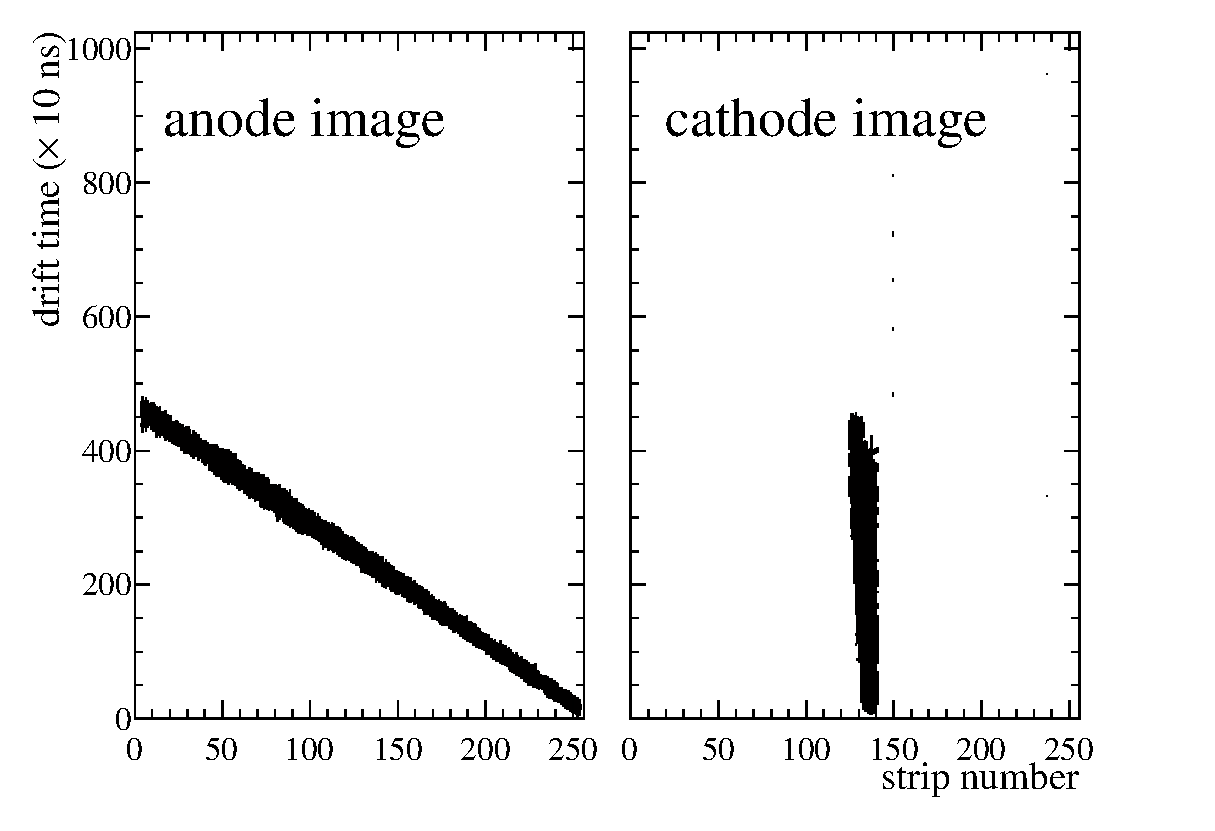
\includegraphics[clip, width=\columnwidth, trim=0 0 50 0]{0210_14.eps}
    \caption{$\alpha$線源によるトラック.}
  \end{subfigure}
  \caption{$\alpha$粒子のトラック [\isoButaneHydro の場合].}
  \label{fig::track_comp_ic4h10_h2}
\end{figure}

\begin{figure}
  \centering
  \begin{subfigure}{0.48\columnwidth}
    \centering
    \includegraphics[clip, width=\columnwidth, trim=0 0 50 0]{iC4H10_1_He_9_0.eps}
    \caption{シミュレーションによるトラック.}
  \end{subfigure}
  \begin{subfigure}{0.48\columnwidth}
    \centering
    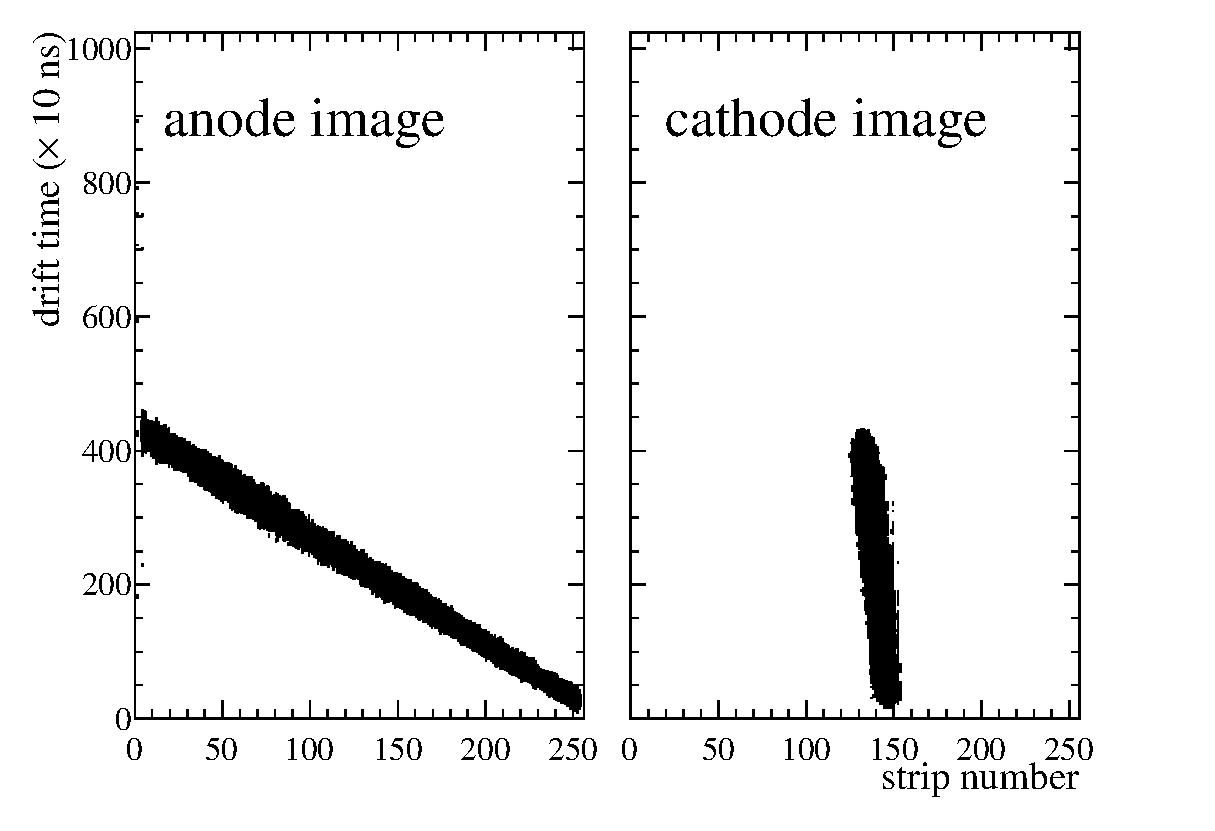
\includegraphics[clip, width=\columnwidth, trim=0 0 50 0]{0176_1.eps}
    \caption{$\alpha$線源によるトラック.}
  \end{subfigure}
  \caption{$\alpha$粒子のトラック [\isoButaneHerium の場合].}
  \label{fig::track_comp_ic4h10_he}
\end{figure}

$\alpha$線源から放出される$\alpha$粒子のエネルギーは平均\SI{4.2}{\mega\electronvolt}である.
一方で,本研究で検出を目指している$0_2^+$状態からの崩壊$\alpha$粒子のエネルギーは数百\si{\kilo\electronvolt}である.
そこで,$\alpha$線源の前に\SI{15}{\micro\metre}のカプトン膜を設置することで$\alpha$粒子のエネルギーを減衰させ,
低エネルギー$\alpha$粒子での測定を行った.
$\alpha$粒子のエネルギーは有感領域と線源の間にある検出ガスによってさらに低下し
TPC の有感領域では約\SI{1}{\mega\electronvolt}となる.
低エネルギー$\alpha$粒子のトラックを
図\ref{fig::track_ch4_loss} [\Methane~(\SI{50}{\hecto\pascal})],
\ref{fig::track_ch4_h2_loss} [\MethaneHydro~(\SI{100}{\hecto\pascal})],
\ref{fig::track_ch4_he_loss} [\MethaneHerium~(\SI{100}{\hecto\pascal})],
\ref{fig::track_ic4h10_h2_loss} [\isoButaneHydro~(\SI{100}{\hecto\pascal})],
\ref{fig::track_ic4h10_he_loss} [\isoButaneHerium~(\SI{100}{\hecto\pascal})] に示す.
コリメータによって$\alpha$線の方向を\ang{30}に制限したため,斜めのトラックとなっている.
シミュレーションでは有感領域の横から\SI{500}{\kilo\electronvolt}の$\alpha$粒子を入射させた.
これらの$\alpha$粒子はMAIKo TPC の有感領域中で停止している.
$\alpha$線源から放出されるエネルギーに広がりがあるため,
エネルギーを完全に一致できていないが,トラックの太さの傾向は再現できている.
\begin{figure}
  \centering
  \begin{subfigure}{0.48\columnwidth}
    \centering
    \includegraphics[clip, width=\columnwidth, trim=0 0 50 0]{a_source_CH4_50_nostr_3.eps}
    \caption{シミュレーションによるトラック.}
  \end{subfigure}
  \begin{subfigure}{0.48\columnwidth}
    \centering
    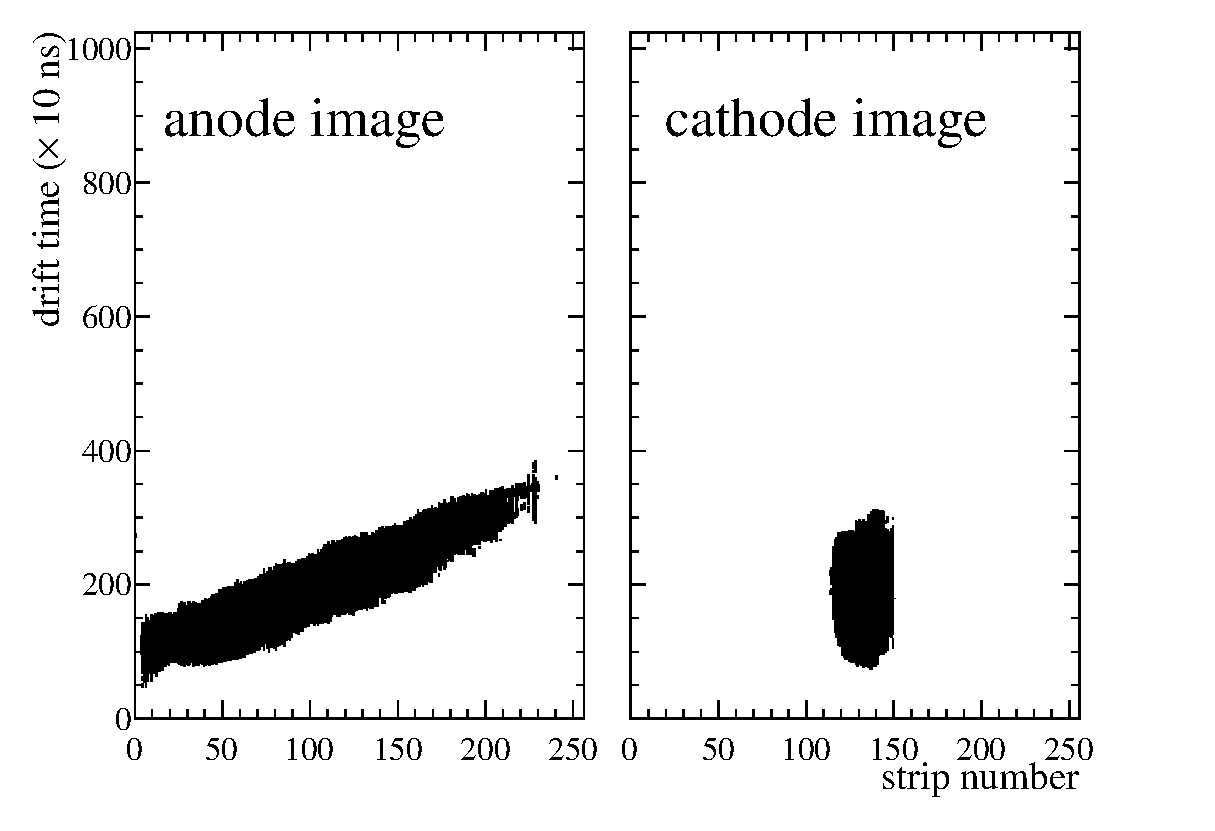
\includegraphics[clip, width=\columnwidth, trim=0 0 50 0]{0146_16.eps}
    \caption{$\alpha$線源によるトラック.}
  \end{subfigure}
  \caption{低エネルギー$\alpha$粒子のトラック [\Methane の場合].}
  \label{fig::track_ch4_loss}
\end{figure}
\begin{figure}
  \centering
  \begin{subfigure}{0.48\columnwidth}
    \centering
    \includegraphics[clip, width=\columnwidth, trim=0 0 50 0]{a_source_CH4_3_H2_7_100_nostr_0.eps}
    \caption{シミュレーションによるトラック.}
  \end{subfigure}
  \begin{subfigure}{0.48\columnwidth}
    \centering
    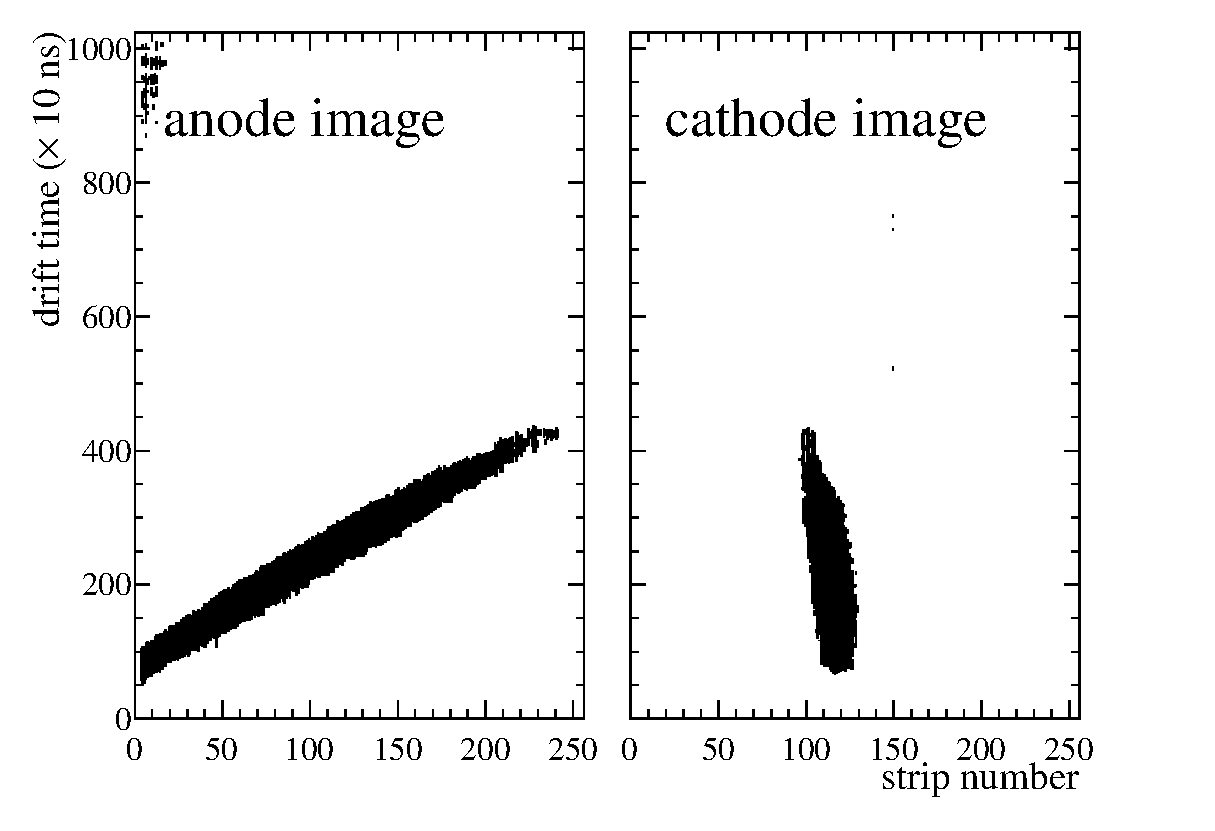
\includegraphics[clip, width=\columnwidth, trim=0 0 50 0]{0209_22.eps}
    \caption{$\alpha$線源によるトラック.}
  \end{subfigure}
  \caption{低エネルギー$\alpha$粒子のトラック [\MethaneHydro の場合].}
  \label{fig::track_ch4_h2_loss}
\end{figure}
\begin{figure}
  \centering
  \begin{subfigure}{0.48\columnwidth}
    \centering
    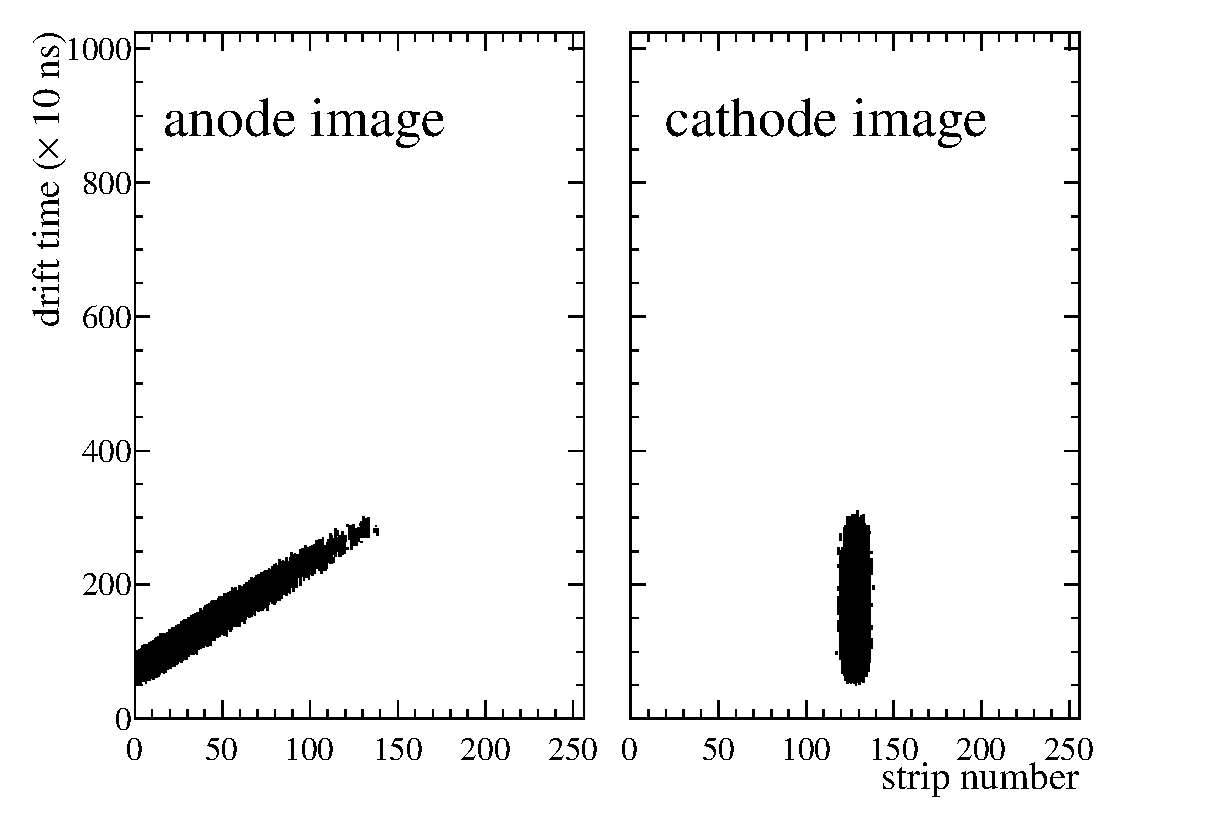
\includegraphics[clip, width=\columnwidth, trim=0 0 50 0]{a_source_CH4_4_He_6_100_nostr_0.eps}
    \caption{シミュレーションによるトラック.}
  \end{subfigure}
  \begin{subfigure}{0.48\columnwidth}
    \centering
    \includegraphics[clip, width=\columnwidth, trim=0 0 50 0]{0204_24.eps}
    \caption{$\alpha$線源によるトラック.}
  \end{subfigure}
  \caption{低エネルギー$\alpha$粒子のトラック [\MethaneHerium の場合].}
  \label{fig::track_ch4_he_loss}
\end{figure}
\begin{figure}
  \centering
  \begin{subfigure}{0.48\columnwidth}
    \centering
    \includegraphics[clip ,width=\columnwidth, trim=0 0 50 0]{a_source_iC4H10_1_H2_9_100_nostr_1.eps}
    \caption{シミュレーションによるトラック.}
  \end{subfigure}
  \begin{subfigure}{0.48\columnwidth}
    \centering
    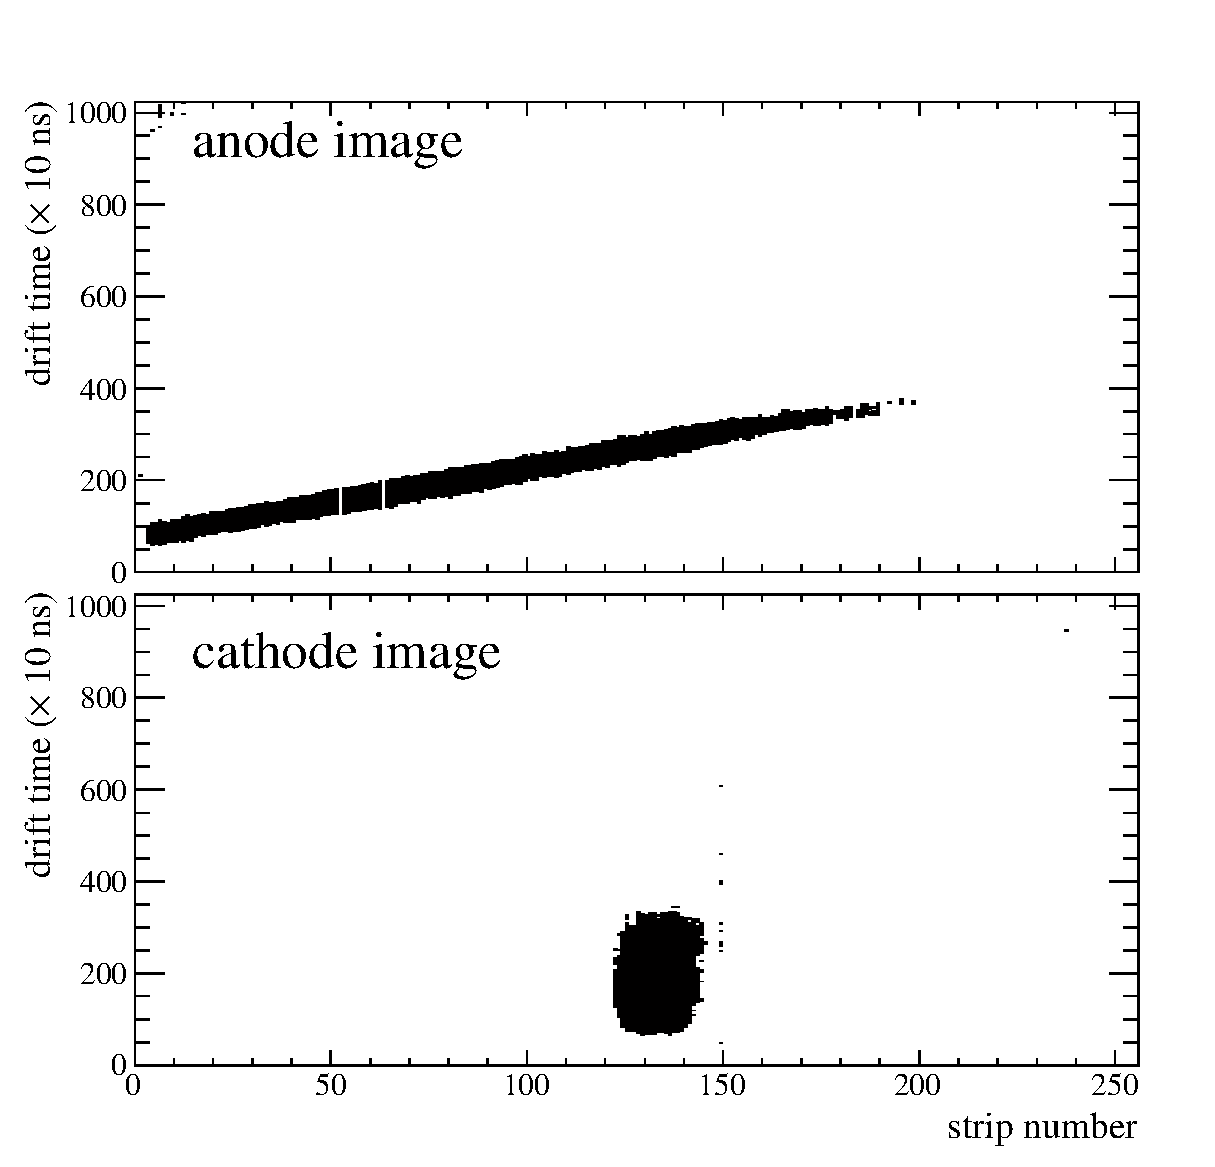
\includegraphics[clip, width=\columnwidth, trim=0 0 50 0]{0211_4.eps}
    \caption{$\alpha$線源によるトラック.}
  \end{subfigure}
  \caption{低エネルギー$\alpha$粒子のトラック [\isoButaneHydro の場合].}
  \label{fig::track_ic4h10_h2_loss}
\end{figure}
\begin{figure}
  \centering
  \begin{subfigure}{0.48\columnwidth}
    \centering
    \includegraphics[clip, width=\columnwidth, trim=0 0 50 0]{a_source_iC4H10_1_He_9_100_nostr_0.eps}
    \caption{シミュレーションによるトラック.}
  \end{subfigure}
  \begin{subfigure}{0.48\columnwidth}
    \centering
    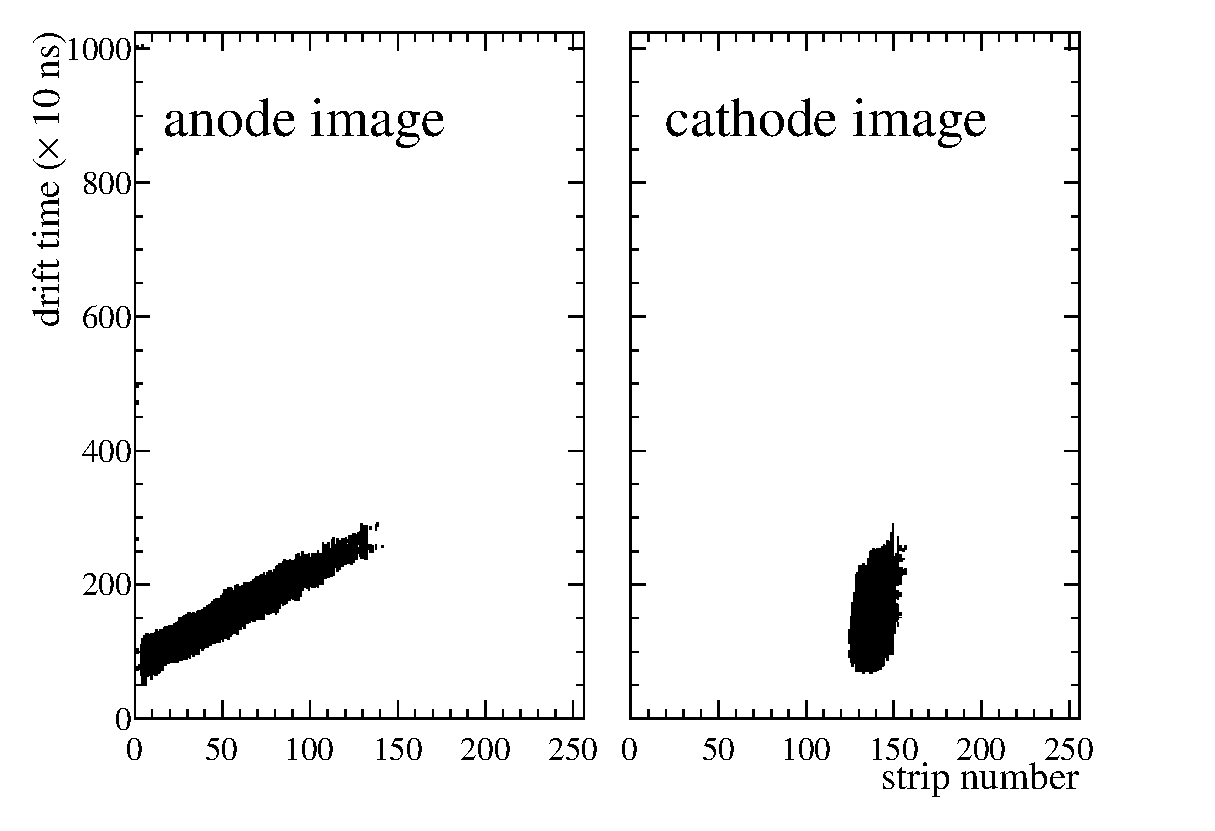
\includegraphics[clip, width=\columnwidth, trim=0 0 50 0]{0203_10.eps}
    \caption{$\alpha$線源によるトラック.}
  \end{subfigure}
  \caption{低エネルギー$\alpha$粒子のトラック [\isoButaneHerium の場合].}
  \label{fig::track_ic4h10_he_loss}
\end{figure}

\section{トリプルアルファ反応のシミュレーション}
\label{sec::triple_alpha_simulation}
$\alpha$線源から放出される$\alpha$粒子のトラックを再現することができたので,
同じ設定で${}^{12}{\mathrm{C}}({\mathrm{n}},{\mathrm{n}}')3\alpha$反応をシミュレーションによって生成した.
このシミュレーションでは以下のように3つの$\alpha$粒子を生成した.
\begin{enumerate}
\item
  ${}^{12}\mathrm{C}$を\SI{14}{\mega\electronvolt}の中性子との非弾性散乱により$0_2^+$状態に励起させる.
  この際,重心系で一様な散乱角で散乱させる.
\item
  ${}^{12}\mathrm{C} (0_2^+)$を$\alpha$粒子と${}^{8}\mathrm{Be}$に位相空間で一様に崩壊させる.
\item
  崩壊してできた${}^{8}\mathrm{Be}$を2つの$\alpha$粒子へ位相空間で一様に崩壊させる.
\end{enumerate}
このようにして得た$\alpha$粒子のトラックを生成する.
トラックの生成方法は前節で述べた通りである.
生成したトラックの例を
図\ref{fig::three_alpha_ch4} [\Methane~(\SI{50}{\hecto\pascal})],
\ref{fig::three_alpha_ch4_h2} [\Methane~(\SI{100}{\hecto\pascal})],
\ref{fig::three_alpha_ch4_he} [\Methane~(\SI{100}{\hecto\pascal})],
\ref{fig::three_alpha_ic4h10_h2} [\isoButaneHydro~(\SI{100}{\hecto\pascal})],
\ref{fig::three_alpha_ic4h10_he} [\isoButaneHerium~(\SI{100}{\hecto\pascal})] に示す.
ここでは,3つのトラックを確認できたイベントを示した.
生成されたイベントの中には$\alpha$粒子のエネルギーと放出角度によっては,
3本のトラックを個別に確認できないイベントも含まれている.
図\ref{fig::not_three_alpha_ch4} [\Methane~(\SI{50}{\hecto\pascal})],
\ref{fig::not_three_alpha_ch4_h2} [\MethaneHydro~(\SI{100}{\hecto\pascal})],
\ref{fig::not_three_alpha_ch4_he} [\MethaneHerium~(\SI{100}{\hecto\pascal})],
\ref{fig::not_three_alpha_ic4h10_h2} [\isoButaneHydro~(\SI{100}{\hecto\pascal})],
\ref{fig::not_three_alpha_ic4h10_he} [\isoButaneHerium~(\SI{100}{\hecto\pascal})] に
2本しかトラックを確認できないイベントの例を示す.

\begin{figure}
  \centering
  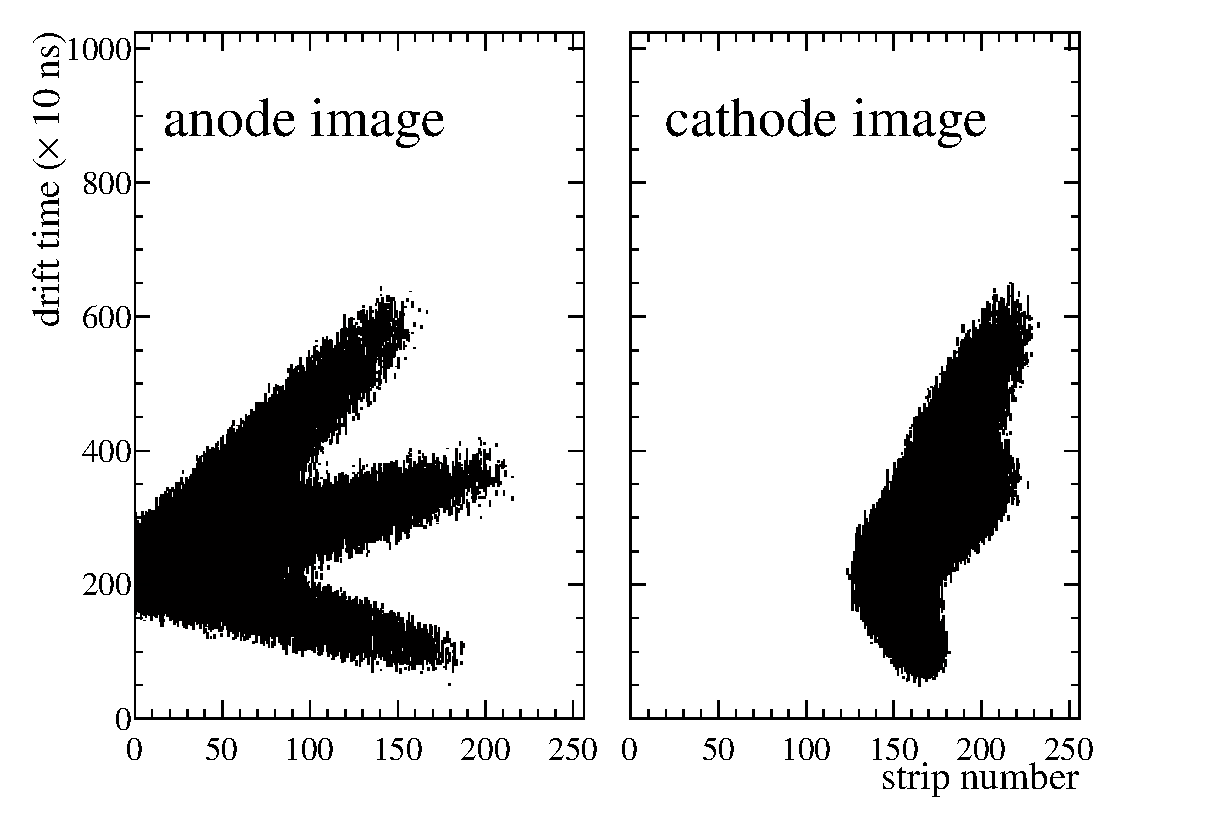
\includegraphics[clip, width=0.8\columnwidth]{10020_7.eps}
  \caption{3$\alpha$のシミュレーション画像 [\Methane の場合].}
  \label{fig::three_alpha_ch4}
\end{figure}

\begin{figure}
  \centering
  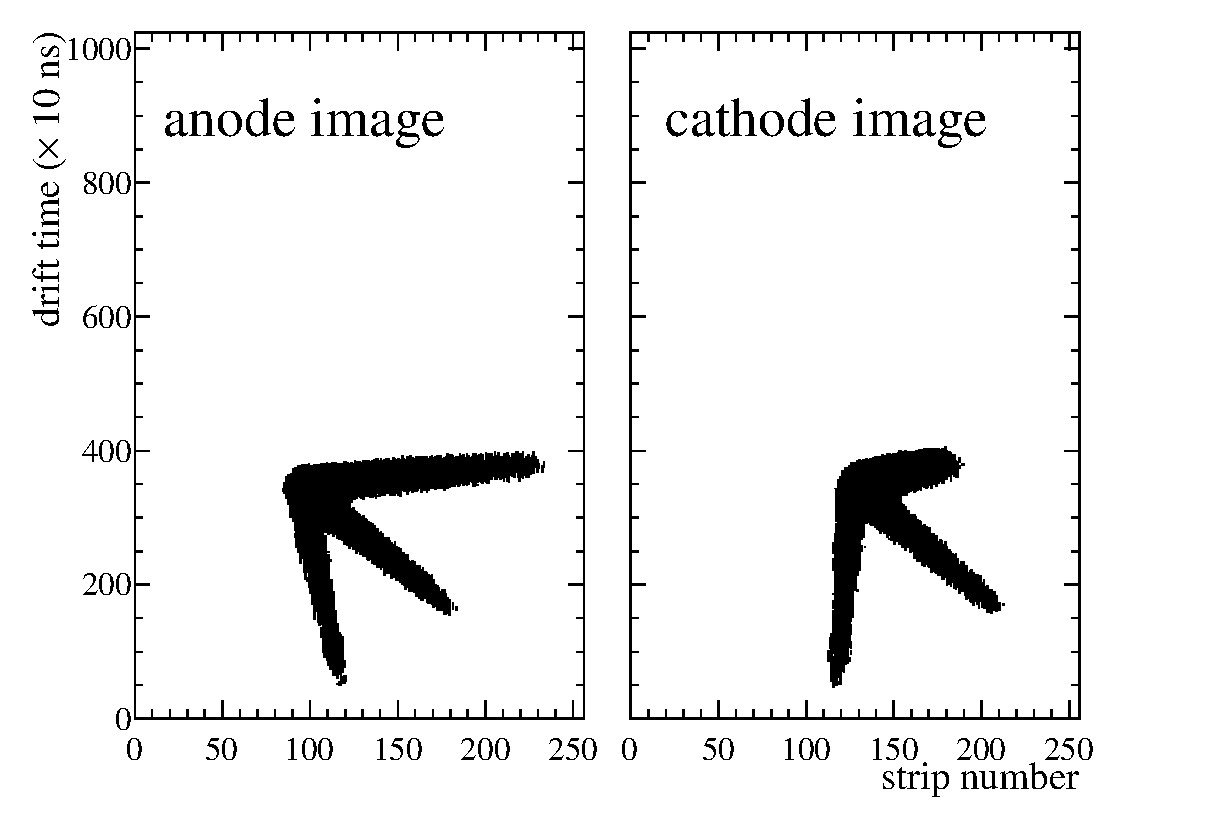
\includegraphics[clip, width=0.8\columnwidth]{10022_15.eps}
  \caption{3$\alpha$のシミュレーション画像 [\MethaneHydro の場合].}
  \label{fig::three_alpha_ch4_h2}
\end{figure}

\begin{figure}
  \centering
  \includegraphics[clip, width=0.8\columnwidth]{10021_5.eps}
  \caption{3$\alpha$のシミュレーション画像 [\MethaneHerium の場合].}
  \label{fig::three_alpha_ch4_he}
\end{figure}

\begin{figure}
  \centering
  \includegraphics[clip, width=0.8\columnwidth]{10024_9.eps}
  \caption{3$\alpha$のシミュレーション画像 [\isoButaneHydro の場合].}
  \label{fig::three_alpha_ic4h10_h2}
\end{figure}

\begin{figure}
  \centering
  \includegraphics[clip, width=0.8\columnwidth]{10023_0.eps}
  \caption{3$\alpha$のシミュレーション画像 [\isoButaneHerium の場合].}
  \label{fig::three_alpha_ic4h10_he}
\end{figure}
\begin{figure}
  \centering
  \includegraphics[clip, width=0.8\columnwidth]{10020_5.eps}
  \caption{2本しかトラックを確認できないイベントの画像 [\Methane の場合].}
  \label{fig::not_three_alpha_ch4}
\end{figure}
\begin{figure}
  \centering
  \includegraphics[clip, width=0.8\columnwidth]{10022_49.eps}
  \caption{2本しかトラックを確認できないイベントの画像 [\MethaneHydro の場合].}
  \label{fig::not_three_alpha_ch4_h2}
\end{figure}
\begin{figure}
  \centering
  \includegraphics[clip, width=0.8\columnwidth]{10021_24.eps}
  \caption{2本しかトラックを確認できないイベントの画像 [\MethaneHerium の場合].}
  \label{fig::not_three_alpha_ch4_he}
\end{figure}
\begin{figure}
  \centering
  \includegraphics[clip, width=0.8\columnwidth]{10024_25.eps}
  \caption{2本しかトラックを確認できないイベントの画像 [\isoButaneHydro の場合].}
  \label{fig::not_three_alpha_ic4h10_h2}
\end{figure}
\begin{figure}
  \centering
  \includegraphics[clip, width=0.8\columnwidth]{10023_32.eps}
  \caption{2本しかトラックを確認できないイベントの画像 [\isoButaneHerium の場合].}
  \label{fig::not_three_alpha_ic4h10_he}
\end{figure}

\end{document}

\documentclass[../master]{subfiles}

\begin{document}

%\chapter{MAIKo TPC で取得したトラックの解析}
\chapter{トラックの解析}
\section{トラック情報の解析の概要}
MAIKo TCP の解析では背景事象の除去とトラック情報の抽出の2つが必要となる.
検出ガスには${}^{12}\mathrm{C}$だけでなく,陽子や${}^{4}\mathrm{He}$が含まれる.
そのため,中性子と陽子,${}^{4}\mathrm{He}$との散乱事象を取り除く必要がある.
陽子や${}^{4}\mathrm{He}$との散乱では複数の荷電粒子が生成されないので,
トラックの本数から識別することができる.
その後,中性子と${}^{12}\mathrm{C}$との散乱事象に対してトラックの情報を抽出する.
トラックの情報は中性子と${}^{12}\mathrm{C}$とが散乱した座標,
$\alpha$粒子が停止した座標である.
anode image から$z, y$座標を,cathode image から$x, y$座標を決定することができる.
$x, z$座標は$\mu$-PIC の信号を検出したstrip のチャンネル番号に\SI{400}{\micro\metre}をかけることで求めることができる.
TPC では,$y$座標を荷電粒子が通過した位置から読み出し面に到達するまでの時間として測定する.
そのため,anode image, cathode image のclock にドリフトスピードをかけることで$y$座標を求めることができる.
このようにして決定したanode image, cathode image の座標を合わせることで,
3次元の座標を求めることができる.

散乱点と停止点の座標から粒子が飛行した方向ベクトルと距離が決定される.
粒子が分かれば,飛行距離から運動エネルギーが決まる.
図\ref{fig::range_to_ene_alpha}に\SI{50}{\hecto\pascal}の\Methane 中での荷電粒子の飛行距離と運動エネルギーの対応を示す.
飛行距離と運動エネルギーの関係はSRIM~\cite{SRIM}を用いて求めた.
SRIM は,荷電粒子がが物質中を通過する際の,イオンの飛程,エネルギーロス等を算出するシミュレーションソフトウェアである.
この対応関係から粒子の運動エネルギーを決定する.
粒子の運動エネルギーを$T$,質量を$m$,単位方向ベクトルを$(dx, dy, dz)$とすると,
粒子の4元運動量は
\begin{equation}
  p =
  \begin{pmatrix}
    E \\ p_{x} \\ p_{y} \\ p_{z}
  \end{pmatrix}
  =
  \begin{pmatrix}
    T + m \\ \sqrt{(T+m)^2 + m^2} dx \\ \sqrt{(T+m)^2 + m^2} dy \\ \sqrt{(T+m)^2 + m^2} dz
  \end{pmatrix}
  \label{eq::momentum_vector}
\end{equation}
となる.
決定した3つの$\alpha$粒子の4元運動量を足し合わせることで,${}^{12}\mathrm{C}$の4元運動量を再構成できる.
このようにして求めた${}^{12}\mathrm{C}$の4元運動量から,
運動エネルギー,散乱角度,励起エネルギーを求めることができる.
\begin{figure}
  \centering
  \includegraphics[clip, width=0.8\columnwidth]{range_to_ene.eps}
  \caption[\Methane (\SI{50}{\hecto\pascal}) 中での荷電粒子 (p, $\alpha$, ${}^{12}\mathrm{C}$) の飛行距離と運動エネルギー.]
          {\Methane (\SI{50}{\hecto\pascal}) 中での荷電粒子 (p, $\alpha$, ${}^{12}\mathrm{C}$) の飛行距離と運動エネルギー.
            この相関はSRIM を用いて求めた.
          }
  \label{fig::range_to_ene_alpha}
\end{figure}

%\subsection{機械学習}
%これまではHough 変換を使って解析を行ってきたが,
%高速に処理をするためにニューラルネットワークを用いた解析方法を開発した.

\section{eye-scanによるトラックの解析}
本研究ではトラックの本数の識別と散乱点,停止点の抽出を人間の目 (eye-scan) で行った.
ここではトラックが3本確認できるイベントを${}^{12}\mathrm{C}(\mathrm{n},\mathrm{n}')3\alpha$イベントとした.
本研究では${}^{12}\mathrm{C}(\mathrm{n},\mathrm{n}')3\alpha$イベントに対して解析を行った.
検出ガスの決定のために,\ref{sec::triple_alpha_simulation}節のシミュレーションで生成したデータのうち,
有感領域中で3つの$\alpha$粒子が停止したイベントに対して解析を行った.

\subsection{解析効率}
実際には${}^{12}\mathrm{C}(\mathrm{n},\mathrm{n}')3\alpha$イベントであっても,
各$\alpha$粒子のエネルギーや放出角度,トラックの太さによっては3つのトラックを区別することができず,
${}^{12}\mathrm{C}(\mathrm{n},\mathrm{n}')3\alpha$イベントとして認識できない場合がある.
そこで,eye-scanによって正しくトラックが3本と認識できる割合(解析効率)を評価する.
eye-scanは各検出ガスについて100 events ずつ行った.
eye-scanによって決定したトラックの本数の割合を表\ref{tab::track_number_ratio}に示す.
表\ref{tab::track_number_ratio}の3本の割合が解析効率となる.
\Methane 単体と\MethaneHerium 以外は約\SI{90}{\percent}の解析効率となっている.
%\begin{table}
%  \centering
%  \caption[シミュレーションデータに対する検出効率.]
%          {シミュレーションデータに対する検出効率.
%            検出効率は全イベントに対して3本のトラックをすべて認識できた割合である.}
%  \label{tab::detection_efficiency}
%  \begin{tabular}{cc}
%    \toprule
%    gas & 検出効率 (\%)\\
%    \midrule
%    \Methane & $55$ \\% \pm 7.42$ \\
%    \MethaneHydro & $91$ \\% \pm 9.54$ \\
%    \MethaneHerium & $78$ \\% \pm 8.83$ \\
%    \isoButaneHydro & $87$ \\% \pm 9.33$ \\
%    \isoButaneHerium & $90$ \\% \pm 9.49$ \\
%    \bottomrule
%  \end{tabular}
%\end{table}
\begin{table}
  \centering
  \caption{eye-scanによって決定したトラックの本数の割合.}
  \label{tab::track_number_ratio}
  \begin{tabular}{cccc}
    \toprule
    gas & 3本 (\si{\percent}) & 2本 (\si{\percent}) & 1本 (\si{\percent}) \\
    \midrule
    \Methane & 55 & 37 & 8 \\
    \MethaneHydro & 91 & 9 & 0 \\
    \MethaneHerium & 78 & 22 & 0 \\
    \isoButaneHydro & 87 & 11 & 2 \\
    \isoButaneHerium & 90 & 10 & 0 \\
    \bottomrule
  \end{tabular}
\end{table}

%\subsection{検出効率の角度依存性}
\subsection{エネルギー分解能}
eye-scanにより決定した$\alpha$粒子の飛行距離の分解能により,エネルギー分解能が決まる.
シミュレーションで粒子を生成した時に決定した$\alpha$粒子の運動エネルギー ($E_{\text{ideal}}$) と
eye-scanによって決定した$\alpha$粒子の運動エネルギー ($E_{\text{eye-scan}}$) の相関を
図\ref{fig::E_corr_ch4}, \ref{fig::E_corr_ch4_h2}, \ref{fig::E_corr_ch4_he},
\ref{fig::E_corr_ic4h10_h2}, \ref{fig::E_corr_ic4h10_he}に示す.
縦軸がシミュレーションで決定した運動エネルギー,横軸がeye-scanで決定した運動エネルギーである.
この相関に対して1次関数 ($E_{\text{ideal}} = p_0\times E_{\text{eye-scan}}+p_1$) でフィットした結果を
表\ref{tab::E_corr_params}にまとめる.
どの検出ガスについても,ほぼ$E_{\text{ideal}} = E_{\text{eye-scan}}$となっている.
\begin{figure}
  \centering
  \begin{minipage}{0.45\columnwidth}
    \centering
    \includegraphics[clip, width=\columnwidth]{E_corr_10020.eps}
    \caption{\Methane の場合の$E_{\text{eye-scan}}$と$E_{\text{ideal}}$の相関.}
    \label{fig::E_corr_ch4}
  \end{minipage}  
\end{figure}
\begin{figure}
  \centering
  \begin{minipage}{0.45\columnwidth}
    \centering
    \includegraphics[clip, width=\columnwidth]{E_corr_10022.eps}
    \caption{\MethaneHydro の場合の$E_{\text{eye-scan}}$と$E_{\text{ideal}}$の相関.}
    \label{fig::E_corr_ch4_h2}
  \end{minipage}
  \begin{minipage}{0.45\columnwidth}
    \centering
    \includegraphics[clip, width=\columnwidth]{E_corr_10021.eps}
    \caption{\MethaneHerium の場合の$E_{\text{eye-scan}}$と$E_{\text{ideal}}$の相関.}
    \label{fig::E_corr_ch4_he}
  \end{minipage}
\end{figure}
\begin{figure}
  \centering
  \begin{minipage}{0.45\columnwidth}
    \centering
    \includegraphics[clip, width=\columnwidth]{E_corr_10024.eps}
    \caption{\isoButaneHydro の場合の$E_{\text{eye-scan}}$と$E_{\text{ideal}}$の相関.}
    \label{fig::E_corr_ic4h10_h2}
  \end{minipage}
  \begin{minipage}{0.45\columnwidth}
    \centering
    \includegraphics[clip, width=\columnwidth]{E_corr_10023.eps}
    \caption{\isoButaneHerium の場合の$E_{\text{eye-scan}}$と$E_{\text{ideal}}$の相関.}
    \label{fig::E_corr_ic4h10_he}
  \end{minipage}
\end{figure}
\begin{table}
  \centering
  \caption{シミュレーションで決定したエネルギーとeye-scan で決定したエネルギーの相関係数.}
  \label{tab::E_corr_params}
  \begin{tabular}{ccc}
    \toprule
    gas & $p_0$ & $p_1$ \\
    \midrule
    \Methane  & 0.985 & \num{1.79e-2} \\
    \MethaneHydro & 0.991 & \num{2.60e-3} \\
    \MethaneHerium  & 0.972 & \num{1.57e-2} \\
    \isoButaneHydro & 0.929 & \num{3.09e-2} \\
    \isoButaneHerium  & 0.962 & \num{1.66e-2} \\
    \bottomrule
  \end{tabular}
\end{table}

$E_{\text{eye-scan}}$をフィットした1次関数 ($f(x)$) で補正したエネルギーと$E_{\text{ideal}}$と
差分を$dE\ (=E_{\text{ideal}}-f(E_{\text{eye-scan}}))$とする.
各検出ガスでの$dE$の分布を図\ref{fig::dE_ch4}, \ref{fig::dE_ch4_h2}, \ref{fig::dE_ch4_he},
\ref{fig::dE_ic4h10_h2}, \ref{fig::dE_ic4h10_he}に,
ガウス分布でフィットした平均と標準偏差を表\ref{tab::energy_resolution}に示す.
エネルギー分解能は,\MethaneHydro の場合に最も良いことが分かる.
%混合ガスの場合,分散は約20 keV となっている.
\begin{figure}
  \centering
  \begin{minipage}{0.45\columnwidth}
    \centering
    \includegraphics[clip, width=\columnwidth]{dE_10020_mod.eps}
    \caption{\Methane の場合の$dE$.}
    \label{fig::dE_ch4}
  \end{minipage}
\end{figure}
\begin{figure}
  \begin{minipage}{0.45\columnwidth}
    \centering
    \includegraphics[clip, width=\columnwidth]{dE_10022_mod.eps}
    \caption{\MethaneHydro の場合の$dE$.}
    \label{fig::dE_ch4_h2}
  \end{minipage}
  \centering
  \begin{minipage}{0.45\columnwidth}
    \centering
    \includegraphics[clip, width=\columnwidth]{dE_10021_mod.eps}
    \caption{\MethaneHerium の場合の$dE$.}
    \label{fig::dE_ch4_he}
  \end{minipage}
\end{figure}
\begin{figure}
  \begin{minipage}{0.45\columnwidth}
    \centering
    \includegraphics[clip, width=\columnwidth]{dE_10024_mod.eps}
    \caption{\isoButaneHydro の場合の$dE$.}
    \label{fig::dE_ic4h10_h2}
  \end{minipage}
  \centering
  \begin{minipage}{0.45\columnwidth}
    \centering
    \includegraphics[clip, width=\columnwidth]{dE_10023_mod.eps}
    \caption{\isoButaneHerium の場合の$dE$.}
    \label{fig::dE_ic4h10_he}
  \end{minipage}
\end{figure}
\begin{table}
  \centering
  \caption{エネルギーの差分の平均と標準偏差.}
  \label{tab::energy_resolution}
  \begin{tabular}{ccc}
    \toprule
    gas & $dE$ (\si{\mega\electronvolt}) & $\sigma_{dE}$ (\si{\mega\electronvolt}) \\
    \midrule
    \Methane  & $1.10\times10^{-2}$ & $3.30\times10^{-2}$  \\
    \MethaneHydro & $1.25\times10^{-3}$ & $2.00\times10^{-2}$ \\
    \MethaneHerium  & $9.30\times10^{-3}$ & $2.37\times10^{-2}$ \\
    \isoButaneHydro  & $4.56\times10^{-3}$ & $2.36\times10^{-2}$ \\
    \isoButaneHerium  & $5.00\times10^{-3}$ & $2.23\times10^{-2}$ \\
    \bottomrule
  \end{tabular}
\end{table}

\subsection{角度分解能}
\subsubsection{極角分解能}
シミュレーションで決定した$\alpha$粒子の極角とeye-scanでの極角の差分を$d\theta$とする.
各検出ガスでの$d\theta$の分布を図\ref{fig::dtheta_ch4}, \ref{fig::dtheta_ch4_h2}, \ref{fig::dtheta_ch4_he},
\ref{fig::dtheta_ic4h10_h2}, \ref{fig::dtheta_ic4h10_he}に,
ガウス分布でフィットした平均とと標準偏差を表\ref{tab::theta_resolution}に示す.
極角分解能は,\Methane 単体の場合に悪いことが分かる.
\begin{figure}
  \centering
  \begin{minipage}{0.45\columnwidth}
    \centering
    \includegraphics[clip, width=\columnwidth]{dtheta_10020_fit.pdf}
    \caption{\Methane を用いた場合の極角の差分.}
    \label{fig::dtheta_ch4}
  \end{minipage}  
\end{figure}
\begin{figure}
  \centering
  \begin{minipage}{0.45\columnwidth}
    \centering
    \includegraphics[clip, width=\columnwidth]{dtheta_10022_fit.pdf}
    \caption{\MethaneHydro を用いた場合の極角の差分.}
    \label{fig::dtheta_ch4_h2}
  \end{minipage}
  \begin{minipage}{0.45\columnwidth}
    \centering
    \includegraphics[clip, width=\columnwidth]{dtheta_10021_fit.pdf}
    \caption{\MethaneHerium を用いた場合の極角の差分.}
    \label{fig::dtheta_ch4_he}
  \end{minipage}
\end{figure}
\begin{figure}
  \centering
  \begin{minipage}{0.45\columnwidth}
    \centering
    \includegraphics[clip, width=\columnwidth]{dtheta_10024_fit.pdf}
    \caption{\isoButaneHydro を用いた場合の極角の差分.}
    \label{fig::dtheta_ic4h10_h2}
  \end{minipage}
  \begin{minipage}{0.45\columnwidth}
    \centering
    \includegraphics[clip, width=\columnwidth]{dtheta_10023_fit.pdf}
    \caption{\isoButaneHerium を用いた場合の極角の差分.}
    \label{fig::dtheta_ic4h10_he}
  \end{minipage}
\end{figure}

\subsubsection{方位角分解能}
シミュレーションで決定した$\alpha$粒子の方位角とeye-scanでの方位角の差分を$d\varphi$とする.
各検出ガスでの$d\varphi$の分布を図\ref{fig::dphi_ch4},\ref{fig::dphi_ch4_h2},\ref{fig::dphi_ch4_he},
\ref{fig::dphi_ic4h10_h2},\ref{fig::dphi_ic4h10_he}に,
ガウス分布でフィットした平均と標準偏差を表\ref{tab::theta_resolution}に示す.
検出ガスに\Methane 単体を用いた時に悪いことが分かる.
\begin{figure}
  \centering
  \begin{minipage}{0.45\columnwidth}
    \centering
    \includegraphics[clip, width=\columnwidth]{dphi_10020_fit.pdf}
    \caption{\Methane を用いた場合の方位角の差分.}
    \label{fig::dphi_ch4}
  \end{minipage}
\end{figure}
\begin{figure}
  \centering
  \begin{minipage}{0.45\columnwidth}
    \centering
    \includegraphics[clip, width=\columnwidth]{dphi_10022_fit.pdf}
    \caption{\MethaneHydro を用いた場合の方位角の差分.}
    \label{fig::dphi_ch4_h2}
  \end{minipage}
  \begin{minipage}{0.45\columnwidth}
    \centering
    \includegraphics[clip, width=\columnwidth]{dphi_10021_fit.pdf}
    \caption{\MethaneHerium を用いた場合の方位角の差分.}
    \label{fig::dphi_ch4_he}
  \end{minipage}
\end{figure}
\begin{figure}
  \centering
  \begin{minipage}{0.45\columnwidth}
    \centering
    \includegraphics[clip, width=\columnwidth]{dphi_10024_fit.pdf}
    \caption{\isoButaneHydro を用いた場合の方位角の差分.}
    \label{fig::dphi_ic4h10_h2}
  \end{minipage}
  \begin{minipage}{0.45\columnwidth}
    \centering
    \includegraphics[clip, width=\columnwidth]{dphi_10023_fit.pdf}
    \caption{\isoButaneHerium を用いた場合の方位角の差分.}
    \label{fig::dphi_ic4h10_he}
  \end{minipage}
\end{figure}

\begin{table}
  \centering
  \caption{角度の差分の平均と標準偏差.}
  \label{tab::theta_resolution}
%  \begin{tabular}{ccccc}
%    \toprule
%    gas & $d\theta$ (\si{\radian}) & $\sigma_{d\theta}$ (\si{\radian}) & 
%    $d\varphi$ (\si{\radian}) & $\sigma_{d\varphi}$ (\si{\radian})\\
%    \midrule
%    \Methane  & $4.64\times10^{-2}$ & $7.79\times10^{-2}$ & $-2.08\times10^{-2}$ & $1.03\times10^{-1}$ \\
%    \MethaneHydro & $2.10\times10^{-3}$ & $2.46\times10^{-2}$ & $-8.28\times10^{-4}$ & $2.47\times10^{-2}$ \\
%    \MethaneHerium  & $3.34\times10^{-3}$ & $2.82\times10^{-2}$ & $-4.46\times10^{-3}$ & $3.40\times10^{-2}$ \\
%    \isoButaneHydro  & $-1.27\times10^{-3}$ & $2.98\times10^{-2}$ & $-3.83\times10^{-3}$ & $2.97\times10^{-2}$ \\
%    \isoButaneHerium & $3.05\times10^{-3}$ & $3.14\times10^{-2}$ & $-3.41\times10^{-3}$ & $2.89\times10^{-2}$ \\
%    \bottomrule
%  \end{tabular}
  \begin{tabular}{ccccc}
    \toprule
    gas & $d\theta$ (degree) & $\sigma_{d\theta}$ (degree) &
    $d\varphi$ (degree) & $\sigma_{d\varphi}$ (degree) \\
    \midrule
    \Methane & $2.66$ & $4.47$ & $-1.19$ & $5.92$ \\
    \MethaneHydro & $1.21\times10^{-1}$ & $1.41$ & $-4.75\times10^{-2}$ & $1.41$ \\
    \MethaneHerium & $1.91\times10^{-1}$ & $1.62$ & $-2.55\times10^{-1}$ & $1.95$ \\
    \isoButaneHydro & $-7.29\times10^{-2}$ & $1.71$ & $-2.20\times10^{-1}$ & $1.70$ \\
    \isoButaneHerium & $1.75\times10^{^1}$ & $1.80$ & $-1.95\times10^{-1}$ & $1.65$ \\
    \bottomrule
  \end{tabular}
\end{table}

\subsection{励起エネルギー分解能}
${}^{12}\mathrm{C}$の励起エネルギーの分解能が悪ければ各励起状態を特定することができない.
シミュレーションでは$0_2^+$状態経由での崩壊を考えているので,
${}^{12}\mathrm{C}(0_2^+)$の励起エネルギーは\SI{7.65}{\mega\electronvolt} となる.
eye-scanで決定した${}^{12}\mathrm{C}^{*}$の不変質量から基底状態の${}^{12}\mathrm{C}$の質量を引くことで励起エネルギーを求め,
\SI{7.65}{\mega\electronvolt} を再構築できるか評価する.
各検出ガスで再構成した励起エネルギーを図\ref{fig::Ex_ch4}, \ref{fig::Ex_ch4_h2}, \ref{fig::Ex_ch4_he},
\ref{fig::Ex_ic4h10_h2}, \ref{fig::Ex_ic4h10_he}, 表\ref{tab::Ex_resolution}に示す.
どの検出ガスにおいても$0_2^+$状態を再構成できていることが分かる.
$0_2^+$状態と隣り合う${}^{12}\mathrm{C}$の励起状態は$2_1^+$の\SI{4.44}{\mega\electronvolt}と
$3_1^-$の\SI{9.64}{\mega\electronvolt}であるので,
分解能も隣り合う励起状態と分けるのに十分良いことも分かる.
\begin{figure}
  \centering
  \begin{minipage}{0.45\columnwidth}
    \centering
    \includegraphics[clip, width=\columnwidth]{Ex_10020_fit.eps}
    \caption{\Methane の場合の${}^{12}\mathrm{C}$の励起エネルギー.}
    \label{fig::Ex_ch4}
  \end{minipage}
\end{figure}
\begin{figure}
  \centering
  \begin{minipage}{0.45\columnwidth}
    \centering
    \includegraphics[clip, width=\columnwidth]{Ex_10022_fit.eps}
    \caption{\MethaneHydro の場合の${}^{12}\mathrm{C}$の励起エネルギー.}
    \label{fig::Ex_ch4_h2}
  \end{minipage}
  \begin{minipage}{0.45\columnwidth}
    \centering
    \includegraphics[clip, width=\columnwidth]{Ex_10021_fit.eps}
    \caption{\MethaneHerium の場合の${}^{12}\mathrm{C}$の励起エネルギー.}
    \label{fig::Ex_ch4_he}
  \end{minipage}
\end{figure}
\begin{figure}
  \centering
  \begin{minipage}{0.45\columnwidth}
    \centering
    \includegraphics[clip, width=\columnwidth]{Ex_10024_fit.eps}
    \caption{\isoButaneHydro の場合の${}^{12}\mathrm{C}$の励起エネルギー.}
    \label{fig::Ex_ic4h10_h2}
  \end{minipage}
  \begin{minipage}{0.45\columnwidth}
    \centering
    \includegraphics[clip, width=\columnwidth]{Ex_10023_fit.eps}
    \caption{\isoButaneHerium の場合の${}^{12}\mathrm{C}$の励起エネルギー.}
    \label{fig::Ex_ic4h10_he}
  \end{minipage}
\end{figure}
\begin{table}
  \centering
  \caption{各ガスで求めた励起エネルギーの平均と標準偏差.}
  \label{tab::Ex_resolution}
  \begin{tabular}{ccc}
    \toprule
    gas & Ex (MeV) & $\sigma_{\text{Ex}}$ (MeV) \\
    \midrule
    \Methane  & 7.63 & $4.91\times 10^{-2}$ \\
    \MethaneHydro & 7.67 & $1.66\times 10^{-2}$ \\
    \MethaneHerium  & 7.67 & $2.05\times 10^{-2}$ \\
    \isoButaneHydro  & 7.67 & $1.75\times 10^{-2}$ \\
    \isoButaneHerium  & 7.67 & $1.90\times 10^{-2}$ \\
    \bottomrule
  \end{tabular}
\end{table}

%\begin{table}
%  \caption{各ガスの解析効率と分解能.それぞれ100 eventsずつeye-scanによって解析を行った.}
%  \label{tab::gas_summary}
%  \begin{tabular}{ccccc}
%    \toprule
%    gas & 解析効率 (\si{\percent}) &
%    $dE\pm\sigma_{dE}$ (\si{\kilo\electronvolt}) &
%    $d\theta\pm\sigma_{d\theta}$ (\si{\milli\radian}) &
%    Ex $\pm\sigma_{\text{Ex}}$ (\si{\mega\electronvolt})\\
%    \midrule
%    \Methane  & 55 &
%    $-4.21\times10^{-3}\pm3.13\times10^{-2}$ & $46.4\pm77.9$ & $7.63\pm4.91\times10^{-2}$ \\
%    \MethaneHydro & 91 & $1.36\times10^{-3}\pm1.97\times10^{-2}$ & $2.10\pm24.6$ & $7.67\pm1.66\times10^{-2}$ \\
%    \MethaneHerium & 78 &
%    $3.75\times10^{-3}\pm2.34\times10^{-2}$ & $3.34\pm28.2$ & $7.67\pm2.05\times10^{-2}$ \\
%    \isoButaneHydro  & 87 & $3.75\times10^{-4}\pm2.80\times10^{-2}$ & $-1.27\pm29.8$ & $7.67\pm1.75\times10^{-2}$ \\
%    \isoButaneHerium  & 90 & $2.14\times10^{-3}\pm2.20\times10^{-2}$ & $3.05\pm31.4$ & $7.67\pm1.90\times10^{-2}$ \\
%    \bottomrule
%  \end{tabular}
%\end{table}

\section{検出ガスの決定}
表\ref{tab::result_summary}に各検出ガスの優劣をまとめた.
$\bigcirc$が優,$\triangle$が可,$\times$が不可を表す.
表の各項目から考えると,\MethaneHydro または
\isoButaneHydro が適すると判断できる.
\MethaneHydro と \isoButaneHydro とで
含まれる${}^{12}\mathrm{C}$の量を比較すると,
\isoButaneHydro の方が4/3倍多い.
よって,検出ガスには\isoButaneHydro~(\SI{100}{\hecto\pascal}) を用いる.
\begin{table}
  \centering
  \caption{各検討項目に対する検出ガスの優劣.標的の量は\Methane に含まれる量を1とした.}
  \label{tab::result_summary}
  \begin{tabular}{ccccc}
    \toprule
    gas & 解析効率 & ディフュージョン & 励起エネルギー分解能 & 標的の量 \\
    \midrule
    \Methane & $\times$ & $\times$ & $\triangle$ & 1 \\
    \MethaneHydro & $\bigcirc$ & $\bigcirc$ & $\bigcirc$ & 0.6 \\
    \MethaneHerium & $\triangle$ & $\triangle$ & $\bigcirc$ & 0.8 \\
    \isoButaneHydro & $\bigcirc$ & $\bigcirc$ & $\bigcirc$ & 0.8 \\
    \isoButaneHerium & $\bigcirc$ & $\triangle$ & $\bigcirc$ & 0.8 \\
    \bottomrule
  \end{tabular}
\end{table}

\end{document}

\chapter{まとめと今後の展望}
\section{まとめ}

\section{本測定に向けて}

\documentclass[../master]{subfiles}

\begin{document}

\chapter*{謝辞}
本研究は多くの方のご助力により成立しています.
指導教官である川畑貴裕教授には,研究の進め方,文章の書き方,発表方法などの多くのことをご指導いただきました.
また,実験の合間にキャッチボールやソフトボールに連れ出していただくなど,
心身ともに健康に研究を行うことができました.
大阪と京都の二重生活でお忙しいにも関わらず,貴重なお時間を私のご指導に当てていただき大変感謝しております.

OKTAVIAN の村田勲教授には,中性子発生装置のことや実験に向けたアドバイスなど多くのご助力を頂き,大変感謝しております.

RCNP の古野達也さんと村田求基さんには,RCNP でMAIKo TPC のテストをしている際に,
お忙しい中で多くのTPC の測定方法やシミュレーションの方法などのアドバイスとご助力をいただきました.
また,食事などに誘って頂きました.
一人で作業をしていることが多かったため,とても感謝しております.
岡本慎太郎くん (M2) には,一緒にMAIKo TPC のテストをやっていただくなど多くの時間をともに過ごしました.
一人では大変な作業を手伝って頂き,大変助かりました.
稲葉健斗さん (D2) には,京都にいるMAIKo TPC のエキスパートとして多くの相談に乗っていただきました.
特にガスやMAIKo TPC の取扱について,なれない私に丁寧にご教授いただきました.
また,一緒にフィットネスに行くことで,健康的な生活を送る一助となりました.
ありがとうございました.
藤川祐輝さん (D1) ,大阪大学の坂梨公亮くん (M1) には,OKTAVIAN での測量などをお手伝いいただき,大変助かりました.
土方佑斗くん (M1) ,延與紫世さん (M1) には,解析の手伝いをして頂き大変助かりました.

同期の関屋涼平くん,原田健志くん,藤井涼平くん,古田悠稀くんとは食事の際にお互いの研究について,
気軽に意見を言い合うことができ大変楽しい時間を過ごしました.
研究室の永江知文教授,成木恵准教授,銭廣十三准教授,村上哲也講師,後神利志助教授,先輩方は
常に研究の進捗を気にかけてくださいました.

最後に,今まで私を支えて頂いた家族や友人に対して深く感謝の意を申し上げます.

\end{document}


\appendix
\chapter{中性子検出器}
\section{液体シンチレータ}
\section{読み出し回路}
\section{n-$\gamma$弁別}
\section{キャリブレーション}


\bibliography{mybibfile}
\end{document}
